
\chapter{Parallel Client Verification}
\label{ch:par}
Symbolic client verification can be used to build a verifier that
validates traffic received from remote clients. This technique can
identify cheating players in multiplayer networked games or identify other types of
malicious behavior in distributed systems. Client verification is
potentially very useful, especially if the validity result can be
computed quickly. Rather than  logging network traffic for
verification off-line, a fast verifier could be configured  to
validate traffic as it arrives at the server. The contributions of
this \paper are motivated by the goal of keeping a  window of attack
that is as small as possible, or in other words, minimizing the time
it takes the verifier to return a validity result for a given message.
The techniques developed thus far in this dissertation
have not achieved efficiency levels that would allow a
verifier to be placed on the critical path of serving client requests. 

At any point in time during verification, there are many possible
paths of exploration; choosing the right path of exploration improves
the latency of the verifier's result. In the previous \paper we
demonstrated that a combination of training data and edit distance
metrics can be used to guide the verifier's exploration. This approach
is successful because it prioritizes exploration on paths that are
more likely to lead to success. However, this algorithm alone cannot
keep pace with all of our client application case studies. For a
long-running or even continuous client-server session, if the average
time to verify a message is greater than the average time between
message arrivals, the verifier falls further and further behind.
In this \paper, we demonstrate a technique to push forward on multiple
paths of exploration in parallel, resulting in significant performance
improvements. 

The ability to keep pace with client traffic is important because it
opens up new avenues for using our client verification technique. If
the verification is fast enough, it can operate \emph{in-line},
allowing each client-to-server message to be verified as being
consistent with the sanctioned client software, before it is processed
by the server. An in-line verification configuration would add some
amount of latency to the client-to-server network traffic, but that
trade-off may be very acceptable in some situations, especially if the
added latency is low or if the cost of invalid command attacks is very
high. \figref{fig:parallel:inline} shows examples of off-line and
in-line verifier configurations; an in-line configuration
can drop a malicious message before it has time to propagate to
the server. The advantages of in-line client verification include:

\begin{itemize}
  \item Elimination of the need for logging network traffic for later
    verification, reducing storage costs.
  \item Better quality of service for other players in multiplayer games;
    cheaters would be removed more quickly, improving the game
    quality for honest players.
  \item Identification of invalid command messages
    \emph{before} they are processed by potentially vulnerable server
    software, crucially saving server operators from potential damage to
    infrastructure or the leakage of private or sensitive data.
\end{itemize}

\begin{figure}[t]
\centering
\subfigure[][Off-line Client Verification]{
\label{fig:parallel:verifier:offline}
\epsfig{file=figures/parallel/verifier_offline.eps, width=0.7\textwidth}
}
\subfigure[][In-line Client Verification]{
\label{fig:parallel:verifier:inline}
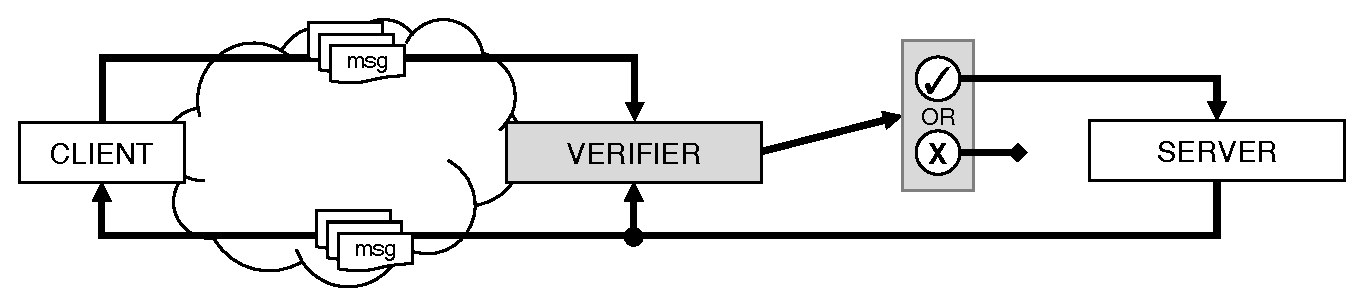
\epsfig{file=figures/parallel/verifier_inline.eps, width=0.7\textwidth}
}
\caption{Off-line and in-line client verification.\label{fig:parallel:inline}}
\end{figure}

\section{Goals and Background}
Our goal is to rapidly identify clients that from the server's
perspective are operating sanctioned client software.
In this \paper we demonstrate that we can achieve
verification results that can keep pace with our case study
applications with a modified version of our verification algorithm. We
describe modifications to our client verification technique to utilize
thread-level parallelism. Although using training data can reduce the
total number of execution states that must be explored, we also wish
to further reduce the time between message arrival and the
verification result. Concurrent exploration can achieve this result.

The outline of the rest of this \paper is as follows.
We will first review the client verification problem and
describe the architecture of our verifier. We then review
multi-threading primitives and describe an algorithm for parallel
client verification in detail. Following that are an overview
of implementation level details and then an evaluation on two
client case studies, \tetrinet and \xpilot.


\subsection{Client Verification Overview}
\label{sec:par:overview}

We now state our assumptions, describe the architecture of the verifier
and the client verification problem.

\subsubsection{Assumptions}
As in the previous chapter,
we are concerned with verifying a client that generates a message
trace, \msg{0}, \msg{1}, $\ldots$, \msg{\msgNmbr}, some sent by the
client and some sent by the server. Furthermore, as before, we assume
the software running on the remote client is single-threaded and that
the verifier is provided with an ordering of messages according to the
client's perspective.

\begin{figure}[t]
\centering
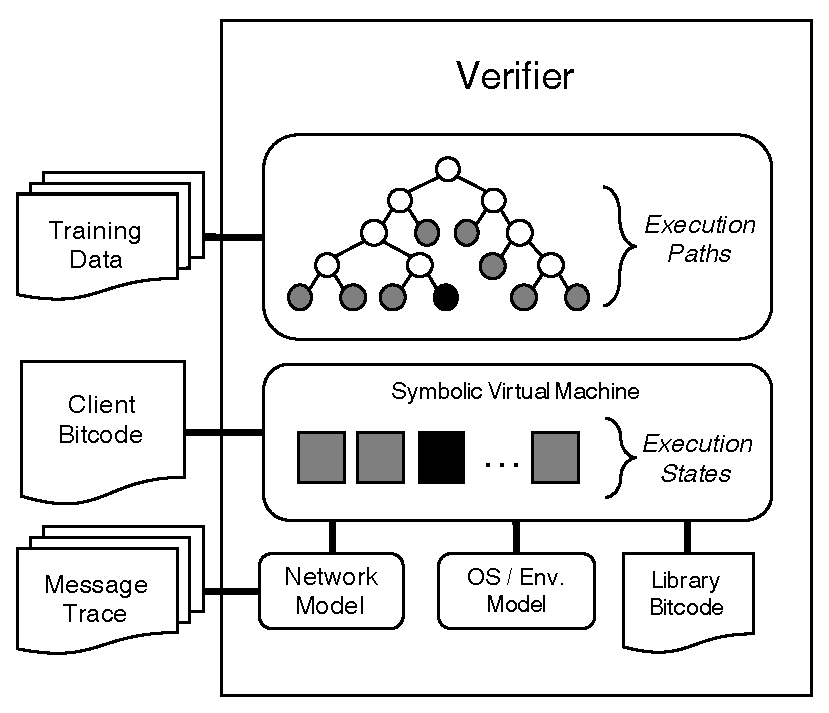
\epsfig{file=figures/parallel/verifier_architecture.eps, width=0.4\columnwidth}
\caption{Verifier Architecture\label{fig:parallel:verifier:arch}}
\end{figure}

\subsubsection{Architecture and Assumptions}
In previous \papers, we have described the verifier architecture shown
in \figref{fig:parallel:verifier:arch}. The verifier operates by
exploring possible execution paths the client may have taken to find a
path that ``explains'' a given message trace. If no such path can be
found, the message trace is declared invalid. The verifier uses
symbolic execution to explore possible client paths. To operate, the
verifier requires three inputs; a message trace, \msgTrace, which will
be verified; the source code for some sanctioned client software,
compiled into an intermediate representation (IR) that can be executed
by a symbolic virtual machine; and a set of training data for
the client bitcode under verification that is used to guide the
selection of possible paths of execution. The message trace is
incrementally fed to the verifier as it arrives at the server and
the verifier outputs if the message trace it has processed thus far can be
explained by an execution path in the software that the client is
expected to be running. 

\subsubsection{Client Verification Definition}
\label{sec:par:definitions}

We formally define the task of the verifier using the same definitions
as \chref{ch:guided}. The verifier's algorithm determines whether
there exists an \textit{execution prefix} of the client that is
\textit{consistent} with the messages $\msg{0}, \msg{1}, \ldots$,
\msg{\msgNmbr}.  Specifically, an execution prefix
\execPrefix{\msgNmbr} is a sequence of client instructions that begins
at the client entry point and follows valid branching behavior in the
client program. We define \execPrefix{\msgNmbr} to be
\textit{consistent} with \msg{0}, \msg{1}, $\ldots$, \msg{\msgNmbr},
if the network \sendInstr and \recvInstr instructions\footnote{We
abbreviate call instructions to POSIX \posixSelect, \posixSend and
\posixRecv system calls (or their functional equivalents) with the
labels \selInstr, \sendInstr and \recvInstr.} in \execPrefix{\msgNmbr}
number $\msgNmbr+1$ and  these network instructions match \msg{0},
\msg{1}, $\ldots$, \msg{\msgNmbr} by direction---i.e., if
\msg{\msgIdx} is a client-to-server message (respectively,
server-to-client message), then the \msgIdx-th network I/O instruction
is a \sendInstr (respectively, \recvInstr)---and if the branches taken
in \execPrefix{\msgNmbr} were possible. Consistency of
\execPrefix{\msgNmbr} with \msg{0}, \msg{1}, $\ldots$, \msg{\msgNmbr}
requires that the conjunction of all symbolic postconditions at
\sendInstr instructions along \execPrefix{\msgNmbr} be satisfiable,
once concretized using the contents of messages \msg{0}, \msg{1},
$\ldots$, \msg{\msgIdx} sent and received on that path. 

The verifier attempts to validate the sequence \msg{0}, \msg{1},
$\ldots$ incrementally, by verifying the sequence \msg{0},
\msg{1}, $\ldots$, \msg{\msgNmbr} starting from an execution prefix
\execPrefix{\msgNmbr-1} found to be consistent with \msg{0}, \msg{1},
$\ldots$, \msg{\msgNmbr-1}, and appending to it an \textit{execution
fragment} that yields an execution prefix \execPrefix{\msgNmbr}
consistent with \msg{0}, \msg{1}, $\ldots$, \msg{\msgNmbr}.
Specifically, an \textit{execution fragment} is a nonempty sequence of
client instructions (i) beginning at the client entry point, a
\selInstr, or a \sendInstr in the client software, (ii) ending at a
\sendInstr or \recvInstr, and (iii) having no intervening \sendInstr
or \recvInstr instructions.  This incremental mechanic is important to
note, as it is the key step in the verification algorithm that we
describe. By using an incremental construction, an entire execution
prefix \execPrefix{\msgNmbr} can be constructed if a given message
trace was produced by a valid client. The verification algorithm
operates as a step-by-step construction of an execution prefix,
because when verification begins, the verifier will only have a single
network message \msg{0}.

\subsubsection{Client Verification Backtracking}
Suppose an execution prefix \execPrefix{\msgNmbr-1} is consistent with
a message trace up to message \msg{\msgNmbr-1}. It is possible for
there to be no execution fragment that can be appended to produce an
execution prefix \execPrefix{\msgNmbr} that is consistent with the
message trace extended by the next message to arrive, \msg{\msgNmbr}.
Intuitively, a path of execution may exercise
client state that precludes future client actions or outputs from
occurring. The verifier incrementally constructs an execution prefix
in an optimistic fashion. In many cases, there is more than one
execution prefix consistent with a message trace, but the verifier
only needs to find one to show that a client is valid. When the
verifier cannot find an execution fragment that can be appended to
\execPrefix{\msgNmbr-1} to produce a \execPrefix{\msgNmbr} consistent
with \msg{0}, \msg{1}, $\ldots$, \msg{\msgNmbr}, then the verifier
backtracks to find a new \execPrefixAlt{\msgNmbr-1} consistent with
\msg{0}, \msg{1}, $\ldots$, \msg{\msgNmbr-1} that can be extended with
an execution fragment to yield a \execPrefixAlt{\msgNmbr} consistent
with \msg{0}, \msg{1}, $\ldots$, \msg{\msgNmbr}.  Only after all such
attempts fail can the client behavior be declared invalid, which may
take substantial time. In practice, an ``invalid'' declaration usually
comes by timeout on the verification process. Our concern in this
\paper is verifying the behavior of \textit{valid} clients quickly,
irrespective of how long it requires to declare an invalid client as
such.

\section{Parallel Client Verification }

We now present a verification algorithm that takes advantage of
thread-level parallelism. At a high level, the main work of
verification is symbolically executing client code to produce an
execution prefix (\secref{sec:par:definitions}) for a given
message sequence. The algorithm that we describe outlines the steps
required to produce an execution prefix \execPrefix{\msgNmbr} from an
execution prefix \execPrefix{\msgNmbr-1}. In practice, many possible
paths of execution need to be explored to produce an execution
fragment. Incomplete paths will be dropped upon reaching unsatisfiable
states and candidate execution fragments will be dropped if the
network action at the end of the fragment is not consistent with the
message trace. Our parallel client verification algorithm
achieves significant improvements in performance by using
thread-level parallelism to explore candidate execution fragments.

\begin{figure}[t]
\centering
\subfigure[][Node data structure]{
\begin{minipage}{0.4\textwidth}
\vspace{15pt}
\begin{tabbing}
\hspace{1em}\=\hspace{9em}\=\kill
\Struct \NodeType $\{$ \\
\> \SymbolicStateType     \> $\sf{state}$; \\
\> \ExecutionFragmentType \> $\sf{path}$; \\
\> \Struct \NodeType      \> $\sf{child[2]}$; \\
$\}$
\end{tabbing}
\vspace{15pt}
\end{minipage}
}
\subfigure[][Node tree with multiple workers attached]{
\centering
\begin{minipage}{0.6\textwidth}
\centering
\epsfig{file=figures/parallel/parallel_node_tree.eps, width=0.84\textwidth}
\vspace{10pt}\end{minipage}
}\
\caption{Node data structure and node tree.
\label{fig:parallel:node}}
\end{figure}

\subsection{Algorithm Definitions}

We now define the data structures used by the algorithm. A 
state \symState{} represents a snapshot of execution in the symbolic
virtual machine, including all constraints (path conditions) and memory
objects, which includes the contents (symbolic or concrete) of
registers, the stack and the heap. The verifier produces state
\symState{\msgNmbr} by symbolically executing the instruction sequence
represented by execution prefix \execPrefix{\msgNmbr}.

The algorithm builds and maintains binary tree,
consisting of \Node objects, shown in \figref{fig:parallel:node}{(a)}.
This tree
is rooted with a state \symState{\msgNmbr-1} and an empty path.
\figref{fig:parallel:node}{(b)} shows an example tree, with a root
node containing \symState{\msgNmbr-1}. (The remaining
node types will be described later in the algorithm description.)
The two children of a node in the tree extend \execPrefix{\msgNmbr-1},
the path represented by \symState{\msgNmbr-1}, 
 through the next symbolic branch (i.e., branch instruction with
 a symbolic condition). One child state holds a constraint
that maintains that the branch condition implies false, and the other
child state holds a constraint that indicates that the branch
condition is true. The algorithm succeeds by finding a fragment with
which to extend \execPrefix{\msgNmbr-1} to yield \execPrefix{\msgNmbr}
if, upon extending a path, it encounters a network I/O instruction
that yields a state with constraints that do not contradict
\msg{\msgNmbr} being the network I/O instruction's message.

We define a set of training data \trainingFrags{} to be a set of
execution fragments and associated message data, observed and
collected via execution of the client prior to verification.
During verification, the verifier selects a subset of execution
fragments $\trainingFrags{\msgNmbr} \subseteq \trainingFrags{}$, for
verification of \msg{\msgNmbr}. The set \trainingFrags{\msgNmbr} is
used prioritize nodes in the node tree rooted at
\symState{\msgNmbr-1}. This prioritization technique is detailed in
\chref{ch:guided}.

\subsection{Key Insights}
The driving goal of our algorithm is to enable concurrent exploration
of multiple states in the node tree. The sooner the algorithm can
explore and then eliminate candidate paths, the sooner it can find a
valid execution fragment. We designed the parallel verification
algorithm to use multiple threads; it uses a single thread to manage
the node tree, a single thread to select the training data subset, and
several worker threads, each assigned to a single node in the node
tree at time. \figref{fig:parallel:node}{(b)} shows an example
assignment of four workers to multiple nodes in a node tree. In our
design and experiments the number of worker threads \workerCount is a
fixed parameter provided to the verifier. Because the verification
task is largely CPU-bound, it is in our experience not beneficial to
use more worker threads than the number of logical CPU cores, and in
some cases, fewer worker threads than cores are necessary. The main
objective of our design is to get ``out of the way'' of the worker
threads. What follows are the high level features of the design.

\begin{itemize}

\item {\bf Concurrent exploration of execution fragments:}
The most important contribution of the algorithm is concurrent
exploration of execution fragments rooted at \symState{\msgNmbr-1}. This
is enabled by a multi-threaded symbolic execution engine (detailed in
\secref{sec:par:klee}). As designed, the algorithm explores only
execution fragments starting from one state \symState{\msgNmbr-1}
corresponding to one execution prefix \execPrefix{\msgNmbr-1}.
Although searching from multiple execution prefixes is not
fundamentally impossible, our implementation of backtracking requires
all worker threads to be exploring fragments in the same node tree.

\item {\bf Non-blocking node tree management:} 
Operations on the node tree operate asynchronously from the worker
threads. This is done so that worker threads do not have to block on
operations that interact with shared data structures. 

\item {\bf Non-blocking training data selection:} 
The parallel verification algorithm extends the method of training
data selection described in \chref{ch:guided}. As before, when
\msg{\msgNmbr} arrives, the verifier selects from a set of execution
fragments \trainingFrags{}, produced during training, that are deemed
likely to be similar to the fragment executed by the client leading up
to it sending or receiving \msg{\msgNmbr}; this subset of execution
fragments is denoted \trainingFrags{\msgNmbr}. Depending on the
size of the training data and granularity of clustering, the selection
of \trainingFrags{\msgNmbr} may take a significant amount of time. The
parallel verification algorithm asynchronously selects
\trainingFrags{\msgNmbr} in a separate thread so that the exploration
from \symState{\msgNmbr-1} is not blocked and can begin before
\trainingFrags{\msgNmbr} is available. Once \trainingFrags{\msgNmbr}
has been computed, the node selection algorithm switches from naive
breadth-first search to an edit-distance search using the selected
subset of execution fragments (\trainingFrags{\msgNmbr}).

 
\end{itemize}

\subsection{Multi-threading primitives}
\label{sec:par:multithreaddefinitions}

The description of our algorithm requires the definition of primitives
used in the dynamic multi-threading model~\cite{cormen09:alg}. These
primitives are $\Spawn$, $\Sync$ and $\Atomic$. The keyword $\Spawn$
must precede a procedure call and has semantics such that the next
statement may continue execution concurrently with the spawned
procedure. In other words, $\Spawn$ indicates the creation of a child
thread that will execute the declared procedure until completion, at
which point the child thread will terminate. The second keyword
$\Sync$ denotes that the parent procedure will wait to proceed to the
next statement until all spawned child threads have finished
execution.  The keyword \Atomic is necessary because, when executing in a
multi-threaded environment, multiple threads may access the same
memory locations at once. In order for concurrent threads to safely
change such a value, a thread that loads and modifies a variable
should execute these operations atomically, in isolation from the rest
the threads. We use the keyword $\Atomic$ in our algorithm description
to indicate that an operation or sequence of operations must execute with
the appearance to other threads of occurring instantaneously. Note
that this is a simplification of the underlying implementation, which
may make use of compare-and-swap operations, mutexes and condition
variables to achieve thread-safe memory operations.


%\algrenewcommand\algorithmicindent{0.5em}%
\begin{figure}[ht]
\begin{minipage}{\textwidth}
\begin{algorithm}[H] % must use H inside minipage
  \caption{Parallel Client Verification}
  %\label{algmultipass}
\begin{algorithmic}[1]
\setalglineno{300}
\Procedure{\parallelVerifyAlg}{\symState{\msgNmbr-1}, 
                               \msg{\msgNmbr}, \trainingFrags{}}
  \label{fig:paralg:parallelVerifyAlg}
  \State $\activeCount \gets 0$
    \Comment{Number of active threads}
    \label{fig:paralg:initWait}
  \State \Atomic $\readyQ \gets \makeNodeQueue()$
    \Comment{Nodes for worker threads to execute}
    \label{fig:paralg:initReady}
  \State \Atomic $\addedQ \gets \makeNodeQueue()$
    \Comment{Nodes created by worker threads}
    \label{fig:paralg:initAdded}
  \State \Atomic $\validState \gets \bot$
    \Comment{Will be set to a valid path if successful}
    \label{fig:paralg:initValid}
  \State \Atomic $\verifyFinished \gets \codeFalse$
    \Comment{Instructs all threads to halt}
    \label{fig:paralg:initFinished}
  \State $\trainingFrags{\msgNmbr} \gets \{\}$
    \Comment{Training for  set \msg{\msgNmbr}}
    \label{fig:paralg:initTraining}
  \State \Spawn \Call{\clusterSelector}{\msg{\msgNmbr}, 
                                        \trainingFrags{}, 
                                        \trainingFrags{\msgNmbr}} 
    %\Comment{Select clusters based on \msg{\msgNmbr}} 
    \label{fig:paralg:spawnClusterSelector}
  \State \Spawn \Call{\nodeScheduler}{\symState{\msgNmbr-1}, 
                                      \trainingFrags{\msgNmbr}, 
                                      \readyQ, \addedQ, 
                                      \activeCount, \verifyFinished}
    %\Comment{Initialize Node Scheduler} 
    \label{fig:paralg:spawnNodeScheduler}
  \For{1 \textbf{to} \workerCount}
    %\Comment{Spawn worker threads} 
    \State \Spawn \Call{\verifyWorker}{\msg{\msgNmbr}, 
                                       \readyQ, \addedQ, 
                                       \activeCount, \verifyFinished, 
                                       \validState}
      \label{fig:paralg:spawnVerifyWorker}
  \EndFor
  \State \Sync
    \Comment{Wait for all child threads} 
    \label{fig:paralg:sync}
  \State \Return \validState
    \Comment{Return result, $\bot$ or \symState{\msgNmbr}}
    \label{fig:paralg:returnValid}
\EndProcedure
\Statex
\end{algorithmic}
\end{algorithm}
\end{minipage}
\caption{Main procedure for parallel client verification.
\label{fig:paralg}}
\end{figure}


\subsection{Details of parallel verification algorithm} 
\label{sec:par:verifydetails}

The algorithm for verifying a client-to-server message using
thread-level parallelism is shown in \figref{fig:paralg}. This
algorithm, denoted \parallelVerifyAlg, takes as input the symbolic
state \symState{\msgNmbr-1} resulting from execution of
\execPrefix{\msgNmbr-1} from the client entry point on message trace
$\msg{0},\ldots,\msg{\msgNmbr-1}$, the next message \msg{\msgNmbr};
and the complete training fragment set \trainingFrags{}.  Its output
is either an execution fragment that can be appended to
\execPrefix{\msgNmbr-1} to make \execPrefix{\msgNmbr} that is
consistent with \msg{0}, $\ldots$, \msg{\msgNmbr}, or no solution 
($\bot$).  The latter case indicates failure and, more specifically,
that there is no execution prefix that can extend
\execPrefix{\msgNmbr-1} to make \execPrefix{\msgNmbr} that is
consistent with \msg{0}, $\ldots$, \msg{\msgNmbr-1}.  This will induce
backtracking to search for another \execPrefixAlt{\msgNmbr-1} that
is consistent with \msg{0}, $\ldots$, \msg{\msgNmbr-1}, which the
verifier will then try to extend to find a \execPrefix{\msgNmbr}
consistent with \msg{0}, $\ldots$, \msg{\msgNmbr}. 

The algorithm operates in a parent thread that spawns $\workerCount+2$
child threads; this includes one thread to select training data, one
thread to manage scheduling of nodes for execution, and \workerCount
worker threads to explore candidate execution fragments.
We outline in detail the operation of algorithm
\parallelVerifyAlg below.

\begin{description}
\item[Initialization:]
First, variables that will be passed to the algorithm sub-procedures
are initialized (Lines
\ref{fig:paralg:initWait}--\ref{fig:paralg:initFinished}). This
includes a counter \activeCount that tracks the number of active
workers (\ref{fig:paralg:initWait}), two empty \NodeType queues
\readyQ  and \addedQ
(\ref{fig:paralg:initWait}--\ref{fig:paralg:initAdded}), an object
\validState that will be set to a valid execution fragment if the algorithm is
successful (\ref{fig:paralg:initValid}) and a boolean \verifyFinished
that will be set to \codeTrue when the algorithm reaches a stop condition
(\ref{fig:paralg:initFinished}). 
%All of these variables may be updated concurrently and thus such operations must use \Atomic.

\item[Training Set Selection Thread:]
Next, on line \ref{fig:paralg:spawnClusterSelector}, a thread is
spawned for \clusterSelector. This procedure selects a set of training
fragments $\trainingFrags{\msgNmbr} \subseteq \trainingFrags{}$ from
the set of all training fragments \trainingFrags{} based on the
contents of the message \msg{\msgNmbr}. The details of this algorithm
are outlined in \chref{ch:guided}. The important change here is that
this algorithm is run in separate thread. We will outline the
intuition behind this choice below. 

\item[Node Selection Thread:] 
The algorithm then spawns a procedure that manages the selection of
nodes to execute next (\ref{fig:paralg:spawnNodeScheduler}). The
parameters to \nodeScheduler are training fragment set
\trainingFrags{\msgNmbr}, node queues \readyQ and \addedQ, counter
\activeCount and boolean \verifyFinished. Procedure \nodeScheduler is
spawned in a child thread so that operations on the node tree do not
block state exploration.

\item[Verification Worker Threads:]
Finally, the algorithm spawns a fixed number of threads that execute
the \verifyWorker procedure (\ref{fig:paralg:spawnVerifyWorker}). This
procedure takes as parameters: network message \msg{\msgNmbr}, node
queues \readyQ and \addedQ, counter \activeCount, boolean
\verifyFinished and execution path \validState. 

\item[Termination:]
Execution is blocked at the call \Sync until all child threads have
exited due to a termination condition, namely $\verifyFinished =
\codeTrue$. After all child threads
have finished the algorithm returns the result \validState, which is
either set by a worker thread to an execution fragment \newPath, that
when appended to \execPrefix{\msgNmbr-1}
is consistent with \msg{0}, $\ldots$, \msg{\msgNmbr} or on
failure, remains undefined $\bot$ as initialized.

\end{description}
\clearpage
%%%%%%%%%%%%%%%%%%%%%%%%%%%%%%%%%%%%%%%%%%%%%%%%%%%%%%%%%%%%%%%%%%%%%%%%
\begin{figure}[ht]
\begin{minipage}{\textwidth}
\begin{algorithm}[H] % must use H inside minipage
\caption{Parallel Client Verification (sub-procedures)}
\begin{algorithmic}[1]
\setalglineno{400}

\Procedure{\nodeScheduler}{\symState{\msgNmbr-1}, \trainingFrags{}, \readyQ, \addedQ, \activeCount, \verifyFinished}
  \label{fig:paralg:nodeScheduler}
  \State $\node \gets \makeNode()$
  \label{fig:paralg:makeRoot}
  \State $\node.\pathField \gets \langle\rangle$; $\node.\stateField \gets \symState{\msgNmbr-1}$
  \label{fig:paralg:initRoot}
  \State $\liveSet \gets \{\node\}$
  \label{fig:paralg:initLiveSet}
  \While{$\verifyFinished =  \codeFalse$}
  \label{fig:paralg:nodeSchedulerWhile}
    \If{$|\liveSet| > 0$ \codeAnd $|\readyQ| < (\workerCount - \activeCount)$}
    \label{fig:paralg:ifEnqueueReady}
      %\State $\displaystyle \node \gets \arg \min_{\nodeAlt \in \liveSet} \min_{\trainingFrag \in \trainingFrags{\msgNmbr}} \min_{\trainingFragAlt \prefixOf \trainingFrag} \editDist(\nodeAlt.\pathField, \trainingFragAlt)$ \\
    \State $\node \gets$ \Call{\selectNode}{\liveSet, \trainingFrags{\msgNmbr}}
    \label{fig:paralg:editDist}
      \State \Atomic $\enqueue(\readyQ, \node)$ 
      \label{fig:paralg:enqueueReady}
    \EndIf
    \While{$|\addedQ| > 0$}
    \label{fig:paralg:ifAdded}
      \State \Atomic $\liveSet \gets \liveSet \cup \{\dequeue(\addedQ)\}$
      \label{fig:paralg:dequeueAdded}
    \EndWhile
    \If{$|\liveSet| = 0$ \codeAnd $|\readyQ| = 0$ \codeAnd $|\addedQ| = 0$ \codeAnd $\activeCount = 0$}
    \label{fig:paralg:ifEmpty}
      \State $\verifyFinished \gets \codeTrue$
      \label{fig:paralg:emptyLive}
    \EndIf
  \EndWhile
\EndProcedure

\State

\Procedure{\verifyWorker}{\msg{\msgNmbr}, \readyQ, \addedQ, \activeCount, \verifyFinished, \validState}
\label{fig:paralg:verifyWorker}
\While{$\verifyFinished = \codeFalse$}
  \label{fig:paralg:verifyWorkerWhile}
  \If{$|\readyQ| > 0$}
  \label{fig:paralg:ifDequeueReady}
    \State \Atomic $\activeCount \gets \activeCount + 1$
    \State \Atomic $\node \gets \tryDequeue(\readyQ)$
    \label{fig:paralg:dequeue}
    \If{$\node \neq \bot$}
      \label{fig:paralg:ifNode}
      \State $\newPath \gets \node.\pathField$ ; $\newState \gets \node.\stateField$ 
      \While{$\isIOInstruction(\newState.\nextInstruction) = \codeFalse$ \codeAnd $\isSymbolicBranch(\newState.\nextInstruction) = \codeFalse$}
        \label{fig:paralg:whileSymEx}
        \State $\newPath \gets \newPath \parallel \langle \newState.\nextInstruction \rangle$
        \label{fig:paralg:extendPath}
        \State $\newState \gets \execStep(\newState)$
        \label{fig:paralg:execStep}
      \EndWhile
      
      \If{$\isIOInstruction(\newState.\nextInstruction) = \codeTrue$}
      \label{fig:paralg:isIOInstruction}
        \If{$((\newState.\constraints\wedge\newState.\nextInstruction.\messageVar= \msg{\msgNmbr}) \not\Rightarrow \codeFalse)$}
          \State $\verifyFinished \gets \codeTrue$
          \State $\validState \gets \newState$
          \label{fig:paralg:returnSuccess}
          \Comment{Success!}
          %\State $\validPath \gets \newPath \parallel \langle \newState.\nextInstruction \rangle$
          %\State \Return 
        \EndIf
      \ElsIf{$\isSymbolicBranch(\newState.\nextInstruction) = \codeTrue$}
        \label{fig:paralg:isSymbolicBranch}
        %\State $\node.\childField{0} \gets \makeNode(\newState, \newState.\nextInstruction.\condition \mapsto \codeFalse)$
        %\State $\node.\childField{0} \gets \makeNode()$
        %\label{fig:paralg:makeChildFalse}
        \State $\node.\childField{0}.\stateField \gets [~\execStep(\newState)~\mid$ $\newState.\nextInstruction.\condition \mapsto \codeFalse~]$
        \label{fig:paralg:branchFalse}
        %\State $\node.\childField{0}.\pathField \gets \newPath \parallel \langle \newState.\nextInstruction \rangle$
        \State $\node.\childField{0}.\pathField \gets \newPath \parallel \langle \node.\childField{0}.\stateField.\nextInstruction \rangle$
        \label{fig:paralg:pathExtendFalse}
        \If{$\node.\childField{0}.\stateField.\constraints \not\Rightarrow \codeFalse$}
        \label{fig:paralg:checkFalse}
          \State \Atomic $\enqueue(\addedQ, \node.\childField{0})$
          \label{fig:paralg:addFalse}
        \EndIf
        %\State $\node.\childField{1} \gets \makeNode(\newState, \newState.\nextInstruction.\condition \mapsto \codeTrue)$
        %\State $\node.\childField{1} \gets \makeNode()$
        %\label{fig:paralg:makeChildTrue}
        \State $\node.\childField{1}.\stateField \gets [~\execStep(\newState)~\mid$ $\newState.\nextInstruction.\condition \mapsto \codeTrue~]$
        \label{fig:paralg:branchTrue}
        \State $\node.\childField{1}.\pathField \gets \newPath \parallel \langle \node.\childField{1}.\stateField.\nextInstruction \rangle$
        \label{fig:paralg:pathExtendTrue}
        \If{$\node.\childField{1}.\stateField.\constraints \not\Rightarrow \codeFalse$}
        \label{fig:paralg:checkTrue}
          \State \Atomic $\enqueue(\addedQ, \node.\childField{1})$
          \label{fig:paralg:addTrue}
        \EndIf

      \EndIf
    \EndIf
    \State \Atomic $\activeCount \gets \activeCount - 1$
  \EndIf

\EndWhile
\label{fig:paralg:mainWhileEnd}
\EndProcedure

\end{algorithmic}
\end{algorithm}
\end{minipage}
\caption{Sub-procedures for parallel client verification.\label{fig:paralg:sub}}
\end{figure}
\clearpage


\subsection{Details of parallel verification algorithm sub-procedures} 
\label{sec:par:nodedetails}

We now describe in further detail the sub-procedures used by
\parallelVerifyAlg and that are shown in \figref{fig:paralg:sub}.
Recall that the parent procedure \parallelVerifyAlg spawns
$\workerCount+2$ child threads which run the procedures
\clusterSelector, \nodeScheduler and \verifyWorker. We omit the
details of \clusterSelector here, it is described in
\chref{ch:guided}.

\subsubsection{Management of nodes in \nodeScheduler}

\parallelVerifyAlg spawns a single thread to run the procedure
\nodeScheduler, shown starting on Line \ref{fig:paralg:nodeScheduler}
of \figref{fig:paralg:sub}. This procedure manages the selection of
nodes to execute next and maintains the flow of nodes between worker
threads. There are two queues of nodes, a ``ready'' queue \readyQ and
an ``added'' queue \addedQ. These queues are shared between the worker
threads and the \nodeScheduler thread. Worker threads pull nodes from
\readyQ and push new nodes onto \addedQ. There is only one scheduler
thread and one or more worker threads producing and consuming nodes
from the queues \readyQ and \addedQ; hence, \readyQ is
a single-producer-multi-consumer queue and \addedQ is a
multi-producer-single-consumer queue. The goal of \nodeScheduler is to
keep \addedQ empty and \readyQ ``full,'' and we will define what we
mean by this below. Nodes are in one of four possible states, either
actively being explored inside \verifyWorker, stored in \readyQ,
stored in \addedQ or stored in \liveSet. A node at the front of
\readyQ is the highest priority node not currently being explored. The
nodes in \addedQ are ``infant'' nodes that have been created by
\verifyWorker threads and need to be added to \liveSet. The remaining
nodes stored in \liveSet are the candidate nodes.

Upon initialization, the procedure \nodeScheduler creates a root node
and adds it to a set of nodes called \liveSet
(\ref{fig:paralg:makeRoot}--\ref{fig:paralg:initLiveSet}). After
initialization, the procedure \nodeScheduler has three cases of
execution. First, the condition on line
\ref{fig:paralg:ifEnqueueReady} checks if \liveSet is non-empty and if
there are more worker threads waiting to execute than nodes in
\readyQ, i.e., the queue \readyQ is not ``full''; if this condition is
true, we call \selectNode (see \chref{ch:guided} for details) and
atomically append the result to \readyQ. Second, if \addedQ is
non-empty, its members are dequeued and added to \liveSet
(\ref{fig:paralg:ifAdded}--\ref{fig:paralg:dequeueAdded}). Finally,
the condition on line \ref{fig:paralg:ifEmpty} is only true if no
worker threads are active, both queues are empty and there are no
remaining states to execute; when this condition is met, all paths of
exploration rooted at \symState{\msgNmbr-1} have been exhaustively
explored and a termination condition has been met. The boolean
\verifyFinished will be set to \codeTrue, forcing all threads to exit.
The parent thread executing \parallelVerifyAlg will return $\bot$ in
this case.

\subsubsection{Building execution fragments in \verifyWorker}

Shown starting on Line \ref{fig:paralg:verifyWorker} of
\figref{fig:paralg:sub}, the procedure \verifyWorker does the main
work of client verification: stepping execution forward in the state \newState of
each node. Like \nodeScheduler, the procedure \verifyWorker runs
inside of a while loop until the value of \verifyFinished is no longer
equal to \codeFalse (\ref{fig:paralg:verifyWorkerWhile}). Recall that
the parent procedure \parallelVerifyAlg spawns multiple instances of
\verifyWorker. Whenever there is a node on the queue \readyQ, the
condition on line \ref{fig:paralg:ifDequeueReady} will be true and the
procedure calls \tryDequeue atomically. Note that even if $|\readyQ| =
0$, multiple instances of \verifyWorker may call \tryDequeue, but only
one will return a node, the rest will retrieve undefined ($\bot$) from
\tryDequeue. 

If \node is not undefined, the algorithm proceeds to execute the state
$\node.\stateField$ and extend the associated path $\node.\pathField$ up
to either the next network instruction (\sendInstr or \recvInstr) or
the next symbolic branch (a branch instruction that is conditioned on
a symbolic variable). The first case, stepping execution on
non-network / non-symbolic-branch instructions, executes in a while
loop on lines \ref{fig:paralg:whileSymEx}--\ref{fig:paralg:execStep}.
The current instruction is appended to the path and the procedure
\execStep is called, which symbolically executes the next instruction
in state \newState. These lines, are where the majority
of the computation work is done by the verifier (see
\figref{fig:time_summary} in \chref{ch:guided}) and
viewed as the ``hot'' path
of the verification algorithm. The ability to concurrently step
execution on multiple states is where the largest performance benefits
of parallelization are achieved. Note that calls to \execStep may
invoke branch instructions, but these are non-symbolic branches. In
the second case, if the next instruction is \sendInstr or \recvInstr
and if the constraints $\newState.\constraints$ accumulated so far
with the symbolic state \newState do not contradict the possibility
that the network I/O message $\newState.\nextInstruction.\messageVar$
in the next instruction $\newState.\nextInstruction$ is \msg{\msgNmbr}
(i.e.,
$(\newState.\constraints\wedge\newState.\nextInstruction.\messageVar =
\msg{\msgNmbr}) \not\Rightarrow \codeFalse$, line
\ref{fig:paralg:isIOInstruction}), then the algorithm sets the
termination value ($\verifyFinished = \codeTrue$) and sets the return
value of the parent function ($\validState \gets \newPath \parallel
\langle \newState.\nextInstruction \rangle$). All other threads of execution
now exit because $\verifyFinished = \codeTrue$ and the parent
procedure \parallelVerifyAlg will return \validState, which is now an
execution fragment that meets the verifier's goals successfully.

In the final case, ($\isSymbolicBranch(\newState.\nextInstruction) =
\codeTrue$), the algorithm is at a symbolic branch. Thus, the branch
condition contains symbolic variables and cannot be evaluated as true
or false in isolation. Using symbolic execution, the algorithm
evaluates both the true branch and the false branch by executing
\newState.\nextInstruction conditioned on the condition evaluating to
\codeFalse (denoted $[~\execStep(\newState) \mid
\newState.\nextInstruction.\condition \mapsto \codeFalse~]$ in line
\ref{fig:paralg:branchFalse}) and conditioned on the branch condition
evaluating to \codeTrue (\ref{fig:paralg:branchTrue}). In each case,
the constraints of the resulting state are checked for consistency
(\ref{fig:paralg:checkFalse}, \ref{fig:paralg:checkTrue}). If either
state is consistent, it is atomically placed onto \addedQ
(\ref{fig:paralg:addFalse}, \ref{fig:paralg:addTrue}).

\subsection{Algorithm summary}
Let us return to \figref{fig:parallel:node}{(b)} from earlier, which
depicts a node tree rooted at \symState{\msgNmbr-1} during the
verification of \msg{\msgNmbr}. The node colored white with a solid
outline represents the \emph{root} node with state
\symState{\msgNmbr-1}. The nodes colored white with dashed outlines,
are the \emph{dead} nodes and represent intermediate states that no
longer exist. A node is dead when it does not reach a success
condition or exits the main if block of \verifyWorker (starting on line
\ref{fig:paralg:ifNode}) without generating any child nodes.
Nodes colored black are the \emph{active} nodes and
are currently being explored by worker threads. Nodes colored dark
gray are in the set \liveSet. If there are worker threads that are ready
to process a node, the highest priority live nodes are in \readyQ,
otherwise live nodes and are either in the set \liveSet. Nodes colored
light grey are  the \emph{infant} nodes and are in \addedQ. We can see
that worker \emph{W4} recently hit a symbolic branch condition and
created two child nodes which were added to \addedQ. The other workers
are likely executing lines
\ref{fig:paralg:whileSymEx}--\ref{fig:paralg:execStep}. 

\section{Multi-threaded KLEE}
\label{sec:par:klee}

Supporting the algorithm described in the previous section requires a
multi-threaded symbolic execution engine. To our knowledge, no current
symbolic execution engines support multi-threaded execution in a
single process. Since
our previous verification tool was built upon \klee,
we modified it to support multi-threaded execution. There were many
small changes made to the code to make it thread-safe, but some of the
major changes include: making the internal reference count class
thread safe, tracking statistics with per-thread objects, adding
critical sections around shared resources, and 
creating separate solver stacks and memory allocators for each worker
thread. 
As a side benefit, this multi-threaded implementation of \klee
can be used outside of client verification and should
enable improved performance for other symbolic execution tasks.

%\begin{figure}[t]
%\centering
%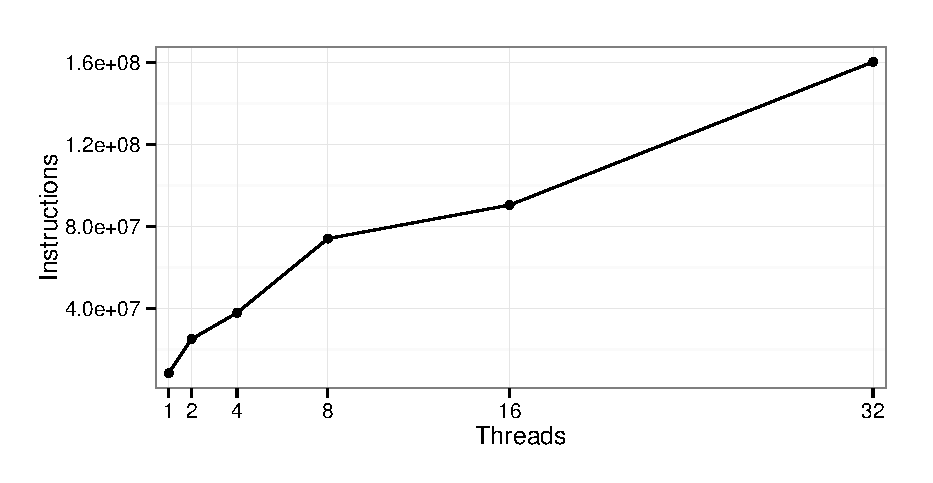
\epsfig{file=figures/parallel/coreutils.eps, width=0.6\columnwidth}
%\caption{Multi-threaded \klee running on \printf from the \coreutils
%suite for five minutes with different numbers of threads.}\label{fig:parallel:coreutils}
%\end{figure}

\section{Evaluation}
\label{sec:par:eval}

We now evaluate the performance of the parallel verification
algorithm. Recall that by design, our verification algorithm has no
false positives --- i.e., if a message trace is declared to be
inconsistent with the sanctioned client software, then it really is.
The only source of false negatives arises from the limited
fidelity of the constraints used to model values returned by
components with which the client software interacts. In these
experiments we make the assumption that the environment modelling is
sound.
We limit our evaluation to \textit{legitimate} message traces since 
our approach is designed to
quickly validate legal behavior in clients that have an unbounded
number of execution paths for exploration.
However, there is no reason that a version of the parallel algorithm 
presented in this \paper could not be applied to the exhaustive
client verification problem from \chref{ch:scv}.

The experiments in this chapter use a multi-threaded version of our
verification tool, built upon KLEE version 1.0\cite{cadar08:klee}, LLVM
3.4\cite{lattner04:llvm} and STP
(rev-940)\cite{ganesh07:stp}.  The experiments were run on system
with 256GB of RAM and 32 3.2GHz processor cores. To evaluate
performance, we applied our parallel algorithm to verify behavior of
legitimate clients of two open-source games from our previous case
studies, namely \xpilot and \tetrinet, which are described in previous
chapters. Evaluation of our parallel verification algorithm requires
message traces for both training and testing.  For \tetrinet, we
generated \tetrinetTraces traces of manual gameplay, each of
\tetrinetTraceLength messages in length (which corresponds to roughly
\tetrinetTraceMins minutes of gameplay).  For \xpilot, we generated
\xpilotTraces traces of manual gameplay, each consisting of
\xpilotTraceLength messages (roughly \xpilotTraceSecs seconds of
gameplay). For our experiments we use the same message traces and
training data from the evaluation section from
\chref{ch:guided}. Note however that these experiments were performed
on a system with a different CPU that has a 10\% higher clock rate.

For each client type, we ran three cross validation experiments over
the message traces with either 1, 8 or 16 worker threads. The training
fragments were clustered with cluster parameter values $\clusters =
\tetrinetFineClusterCount$ and $\clusters = \xpilotFineClusterCount$
for \tetrinet and \xpilot, respectively. These parameters ensured a
single training fragment per cluster and corresponds to the
``default'' configuration used in \chref{ch:guided}. These experiments
do not include results using the ``hint'' configuration, because as we
will see, when using the parallel verification technique, client-side
modification to provide hints to the verifier is not necessary. 
Although the experiments in our evaluation use the same data, the
single worker experiments in this \paper gain the benefits of separate
threads for the \nodeScheduler and \clusterSelector procedures and the
increased clock rate of our experiment platform.

In our evaluation we observe two data points for each \msg{\msgNmbr} in
a message trace, verification \textit{cost} and verification
\textit{delay}. The verification cost for message \msg{\msgNmbr},
denoted \cost{\msgNmbr}, accounts for all time spent in
$\parallelVerifyAlg(\symState{\msgNmbr-1}$, \msg{\msgNmbr},
$\trainingFrags{})$. This is measured as the wall-clock time that
the algorithm takes to determine that \msg{\msgNmbr} is
valid.\footnote{If backtracking occurs, that time is included in the
verification time of the associated message index, i.e., the verification time
for \msg{\msgNmbr} may include the total wall clock time of more than
one instance of $\parallelVerifyAlg$.} Note that the verification time
represents work done concurrently and doesn't represent the total
summation of CPU time across multiple cores. Our second data point
for evaluation is the verification \textit{delay}, which is the delay
in time between the arrival of message \msg{\msgNmbr} at the server
(where a server-to-client message ``arrives'' when it is sent) and the
discovery of an execution prefix \execPrefix{\msgNmbr} that is
consistent with \msg{0}, $\ldots$, \msg{\msgNmbr}.  Delay differs from
verification time by representing the fact that verification for
\msg{\msgNmbr} cannot begin until after verification for \msg{\msgNmbr-1}
completes.  The methods for calculating verification cost and delay
are formally defined in \secref{sec:guided:eval} of \chref{ch:guided}.

\subsection{Case Study: \tetrinet}

\begin{figure}[ht]
\centering
\small
\begin{tabular}{|r|rrr|rrr|}
\hline
& \multicolumn{3}{c|}{Cost (s)} & \multicolumn{3}{c|}{Delay (s)} \\
\hline
\workerCount & 16 & 8 & 1 & 16 & 8 & 1 \\ 
\hline
% & ed-16\_Time & ed-8\_Time & ed-1\_Time & ed-16\_Delay & ed-8\_Delay & ed-1\_Delay \\ 
Min       & 0.0007  & 0.0003  & 0.0001   & 0.0008  & 0.0003  & 0.0001 \\
Max       & 12.1548 & 16.6219 & 100.8736 & 13.1708 & 22.7357 & 337.01 \\
Median    & 0.0368  & 0.0370  & 0.0321   & 0.0489  & 0.0484  & 17.946 \\
Mean      & 0.1287  & 0.1622  & 1.5859   & 0.3975  & 0.6361  & 57.137 \\
%Variance & 0.5796  & 1.0747  & 79.0533  & 2.2025  & 5.4354  & 6040.1192 \\
Std. Dev. & 0.7613  & 1.0367  & 8.8912   & 1.4841  & 2.3314  & 77.718 \\
\hline
\end{tabular}
\caption{Summary statistics for \tetrinet results
\label{fig:tetrinet:parallel:stats}}
\end{figure}

\figref{fig:tetrinet:parallel:stats} shows summary statistics for the
parallel verification algorithm on the \tetrinet experiments and shows
both verification costs and delays for 16-worker, 8-worker and
1-worker configurations.
These results  were obtained by a \tetrinetTraces-fold cross
validation of the \tetrinet traces; i.e., in each test, one of the
traces was selected for testing, and the remainder were used for
training. Each row in \figref{fig:tetrinet:parallel:stats}
is a measure of values (costs or delays) observed over all \tetrinetTraces
experiments.
The mean verification cost per message, regardless of the
number of threads used, is easily beneath the inter-message delay of
roughly \tetrinetInterMessageDelay. As an optimization over results in
\chref{ch:guided}, we can see that parallelization of the verification
algorithm allows us to drop the mean verification cost from
$1.59\secs$ using a single worker thread to $130\msecs$ when using the 16-thread
configuration. If the verifier was placed in-line, this might be an
acceptable overhead on average to add to the processing of network data. However
the maximum verification time of $12.15\secs$ is greater than
the average inter-message delay of \tetrinetInterMessageDelay and
would not be an acceptable amount of latency to add to the
client-server communication. Looking at the Delay columns in
\figref{fig:tetrinet:parallel:stats} we can see that the max delay is
25X less in the 16-worker configuration than in the 1-worker
configuration.

\figref{fig:tetrinet:parallel:time} shows the distribution of
verification cost per message, binned into ten-message bins, across
all \tetrinetTraces traces.  The boxplot labeled ``0'' shows the
distribution of verification times for messages
$\msg{0},\ldots,\msg{9}$ in the \tetrinetTraces traces. In each
boxplot, the ``box'' shows the first, second (median) and third
quartiles, and with whiskers extending to $\pm 1.5$ times the
interquartile range.  Additional outlier points are shown as dots.
Overlaid on each boxplot is a diamond ($\Diamond$) that shows the
average of the data points. In \figref{fig:tetrinet:parallel:time} we can see how additional
worker threads reduce the verification costs. We can also see that it
is the outlier points that dominate the overall time spent in the
verifier, with bands at $90\secs$, $14\secs$ and $10\secs$ for the
three configurations.
Comparing the 1-worker and 16-worker configurations, the performance
multiplier is roughly 9, rather than 16. Our implementation does not
achieve a ``perfect'' speed-up when adding additional workers and
there are several factors that may be at play.
First, a single outlier can represent
verification in multiple node trees due to backtracking. 
Although $2.5\%$ of \tetrinet messages required backtracking, there
is not a direct correlation between existence of backtracking and
higher verification cost. Nevertheless, a round with backtracking cannot
exploit multiple workers as efficiently as possible because early in
the exploration of a node tree because there are more fewer live nodes than
workers available. Second, there is some overhead in our
implementation and as we add more threads there is a added cost to
access shared resources. We attempted to minimize this as much as
possible in our design. 

\figref{fig:tetrinet:parallel:delay} plots the distributions of
per-message verification \textit{delay} between the arrival of message
\msg{\msgNmbr} at the server and the discovery of an execution prefix
\execPrefix{\msgNmbr} that is consistent with \msg{0}, $\ldots$,
\msg{\msgNmbr}.  Delay (\figref{fig:tetrinet:parallel:delay}) differs
from verification cost (\figref{fig:tetrinet:parallel:time}) by
representing the fact that verification for \msg{\msgNmbr} cannot
begin until after that for \msg{\msgNmbr-1} completes.  So, for
example, the rightmost boxplot in each graph provides insight into how
long after the completion of the message trace (in real time) that it
took for verification for the whole trace to complete. We note that
for the multi worker configurations of 8 and 16 workers, verification
is able to keep pace with gameplay and never accumulates delay over
the course of verification. The median of the rightmost boxplot is
virtually zero. Even if verification falls behind at some point in the
game, it always catches up because of the gap between message arrival
times. This indicates that the verifier needs only a fixed sized
buffer of network messages to manage a long-running verification
session. We see that in \figref{fig:tetrinet:parallel:delay}{c}, which
shows the single worker configuration, verification delay lags behind
message arrival times by more than $60\secs$ by the end of a
\tetrinetTraceLength-message trace in the average case. 

\clearpage
\begin{figure}[th]
\centering
\begin{tabular}{c}
%\subfigure[][16 worker threads, $\clusters = \tetrinetFineClusterCount$]{
\subfigure[][$\workerCount = 16$]{
\label{fig:tetrinet:time:parallel_16_default_fine}
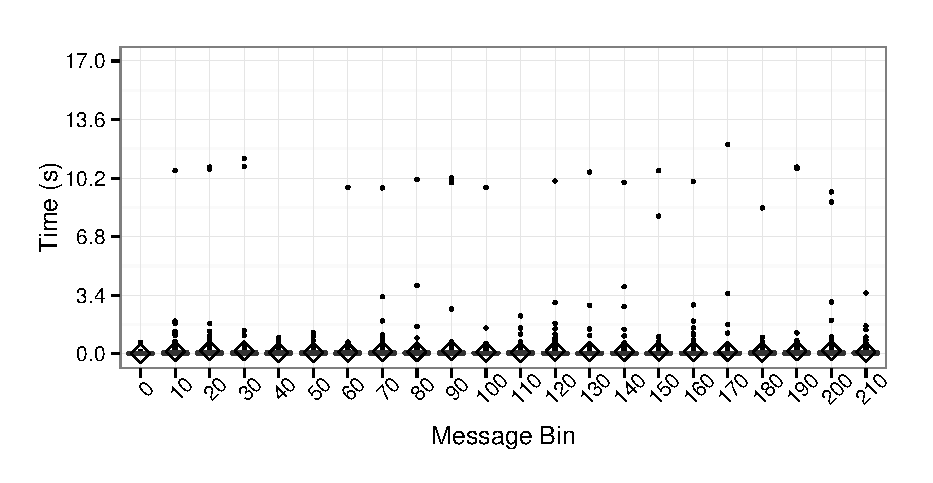
\epsfig{file=figures/parallel/tetrinet_ed-16_Time_boxplot_bar_alt.eps,width=0.6\columnwidth}
} \\[-5pt]
%\subfigure[][8 worker threads, $\clusters = \tetrinetFineClusterCount$]{
\subfigure[][$\workerCount = 8$]{
\label{fig:tetrinet:time:parallel_8_default_fine}
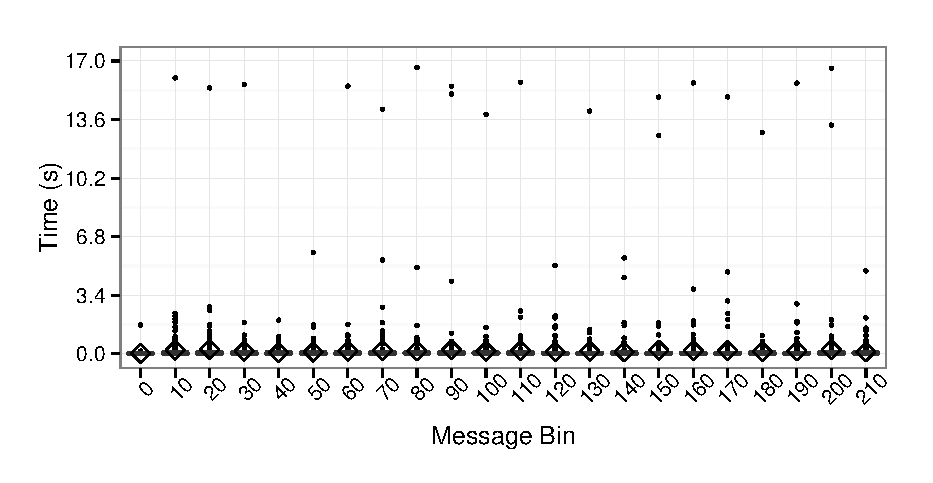
\epsfig{file=figures/parallel/tetrinet_ed-8_Time_boxplot_bar_alt.eps,width=0.6\columnwidth}
} \\[-5pt]
%\subfigure[][1 worker thread, $\clusters = \tetrinetFineClusterCount$]{
\subfigure[][$\workerCount = 1$]{
\label{fig:tetrinet:time:parallel_1_default_fine}
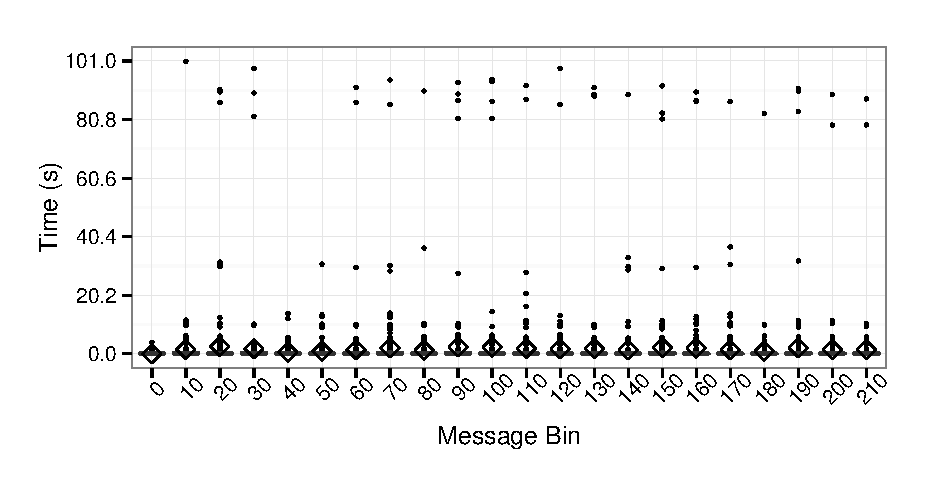
\epsfig{file=figures/parallel/tetrinet_ed-1_Time_boxplot_bar_alt.eps,width=0.6\columnwidth}
}\end{tabular}
\caption[\tetrinet parallel verification costs.]{\tetrinet parallel verification costs.
Cross-validation over \tetrinetTraces traces.  Boxplot at \xval shows
verification costs for messages \msg{\xval}, $\ldots$, \msg{\xval+9}
in each trace (after training on the other traces).  ``$\Diamond$''
shows the average.}
\label{fig:tetrinet:parallel:time}
\end{figure}
\clearpage

\clearpage
\begin{figure}[th]
\centering
\begin{tabular}{c}
%\subfigure[][16 threads, $\clusters = \tetrinetFineClusterCount$]{
\subfigure[][$\workerCount = 16$]{ 
\label{fig:tetrinet:delay:parallel_16_default_fine}
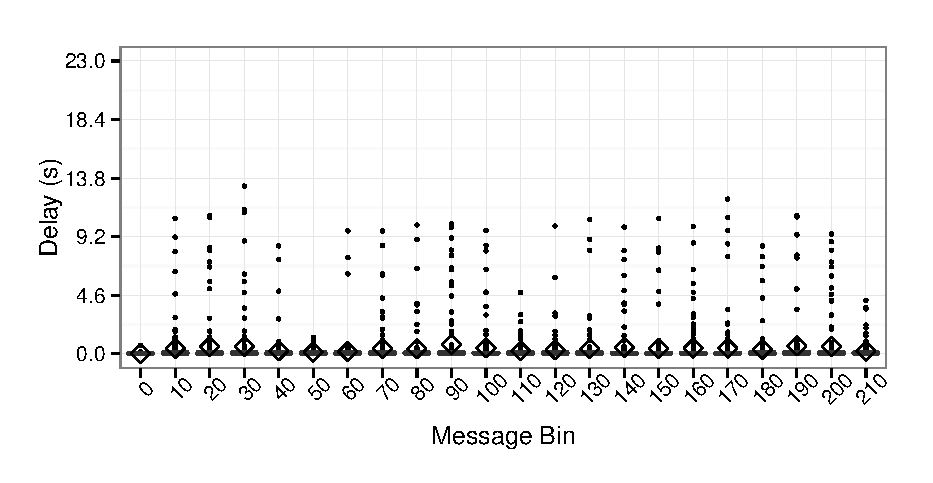
\epsfig{file=figures/parallel/tetrinet_ed-16_Delay_boxplot_bar_alt.eps,width=0.6\columnwidth}
} \\[-5pt]
%\subfigure[][8 threads, $\clusters = \tetrinetFineClusterCount$]{
\subfigure[][$\workerCount = 8$]{
\label{fig:tetrinet:delay:parallel_8_default_fine}
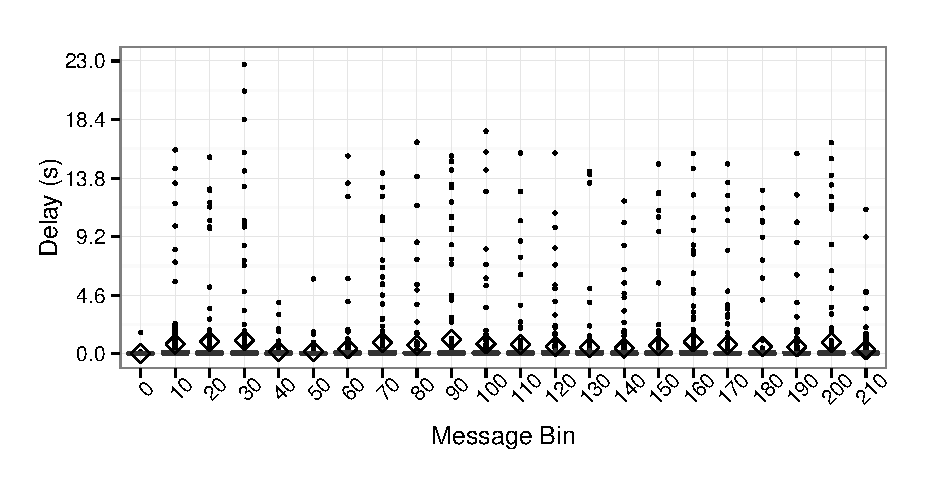
\epsfig{file=figures/parallel/tetrinet_ed-8_Delay_boxplot_bar_alt.eps,width=0.6\columnwidth}
} \\[-5pt]
%\subfigure[][Single-threaded, $\clusters = \tetrinetFineClusterCount$]{
\subfigure[][$\workerCount = 1$]{
\label{fig:tetrinet:delay:parallel_1_default_fine}
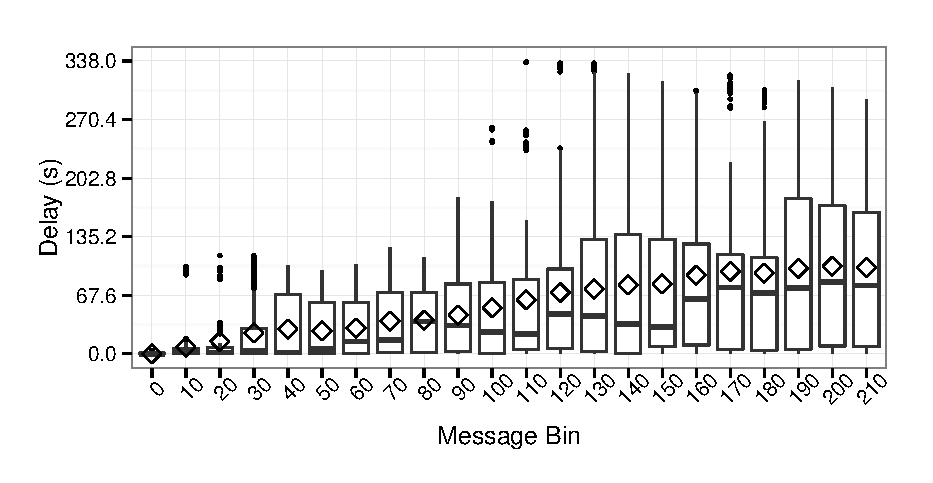
\epsfig{file=figures/parallel/tetrinet_ed-1_Delay_boxplot_bar_alt.eps,width=0.6\columnwidth}
}\end{tabular}
\caption[\tetrinet parallel verification delays.]{\tetrinet parallel verification delays.
Cross-validation over \tetrinetTraces traces.  Boxplot at \xval shows
verification delays for messages \msg{\xval}, $\ldots$, \msg{\xval+9}
in each trace (after training on the other traces).  ``$\Diamond$''
shows the average.}
\label{fig:tetrinet:parallel:delay}
\end{figure}
\clearpage

\subsection{Case Study: \xpilot}

\begin{figure}[ht]
\centering
\small
\begin{tabular}{|r|rrr|rrr|}
\hline
& \multicolumn{3}{c|}{Cost (s)} & \multicolumn{3}{c|}{Delay (s)} \\
\hline
\workerCount & 16 & 8 & 1 & 16 & 8 & 1 \\ 
%& ed-16\_Time & ed-8\_Time & ed-1\_Time & ed-16\_Delay & ed-8\_Delay & ed-1\_Delay \\ 
\hline
Min        & 0.0004 & 0.0004 & 0.0001 & 0.0025 & 0.0022 & 0.0023 \\
Max        & 0.7071 & 0.4966 & 5.4948 & 1.1990 & 1.5294 & 122.85 \\
Median     & 0.0164 & 0.0168 & 0.0122 & 0.0205 & 0.0250 & 29.869 \\
Mean       & 0.0205 & 0.0213 & 0.0658 & 0.0754 & 0.0791 & 32.740 \\
%Variance  & 0.0006 & 0.0004 & 0.0186 & 0.0173 & 0.0156 & 585.0364 \\
Std. Dev.  & 0.0237 & 0.0198 & 0.1364 & 0.1313 & 0.1248 & 24.187 \\
\hline
\end{tabular}
\caption{Summary statistics for \xpilot results
\label{fig:xpilot:parallel:stats}}
\end{figure}


\figref{fig:xpilot:parallel:stats} shows the summary statistics of
the experiments on \xpilot, for verification cost and delay -- 
using 16-worker, 8-worker and 1-worker configurations.
\xpilot poses a different challenge than \tetrinet for verification 
because the message rate is so fast. The tests described here use an \xpilot
configuration that resulted in an average of \xpilotMsgsPerSec
messages per second or an average inter-message
time of \xpilotInterMessageDelay. Nevertheless, with our parallel
verification technique, we can achieve a mean verification
cost of only $20\msecs$ and return a verification result in less
than $0.71\secs$ for all messages in our experiments. 
The multi-worker configurations are both more than $3\times$ faster
on average than the single worker configuration.
For the 16-worker configuration, the verifier is on average
only $75\msecs$ behind ($1.19\secs$ in the worst case), whereas when
using only a single-worker, verification delay is on average
$32.7\secs$ and over 2 minutes in the worst case.
These results demonstrate that in-line verification is feasible
and would add minimal latency in the average case. However,
adding $1.19\secs$ of latency in the worst case would not be acceptable
for fast-paced gameplay.

In \figref{fig:xpilot:parallel:time}, the verification costs for
\xpilot are shown for the three worker configurations across the
message traces. Each boxplot in \figref{fig:xpilot:parallel:time}
represents $100 \times \xpilotTraces$ points.
Despite a mean verification cost of $75\msecs$ when using
a single worker thread, the fast pace of \xpilot makes it difficult 
for verification to keep pace with the game.  This effect is shown in
\figrefi{fig:xpilot:parallel:delay}{c}.  
However, by increasing the number of worker threads, we can see that
in the 16-worker and 8-worker configurations, verification delay
never significantly falls behind and could use only a fixed
buffer of messages for verification in long running sessions.

\clearpage
\begin{figure}[th]
\centering
\begin{tabular}{c}
%\subfigure[][16 threads, $\clusters = \xpilotFineClusterCount$]{
\subfigure[][$\workerCount = 16$]{
\label{fig:xpilot:time:parallel_16_default_fine}
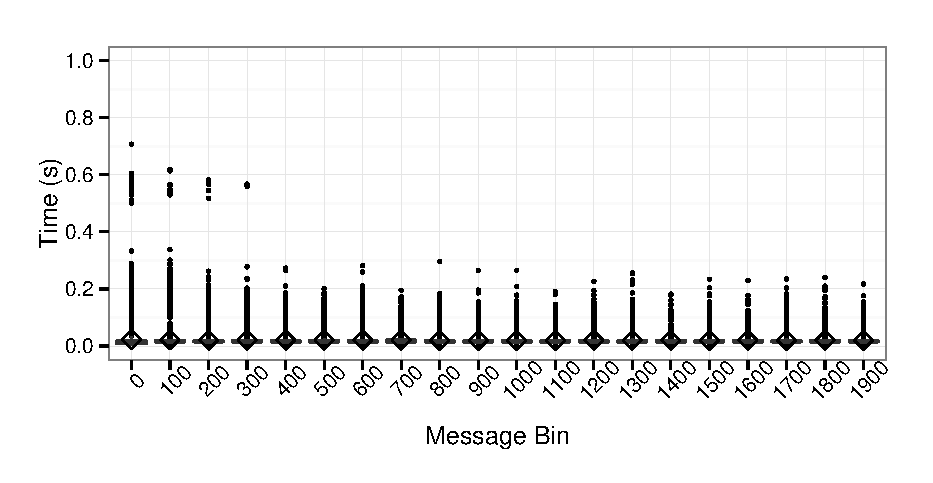
\epsfig{file=figures/parallel/xpilot_ed-16_Time_boxplot_bar_alt.eps,width=0.6\columnwidth}
} \\[-5pt]
%\subfigure[][8 threads, $\clusters = \xpilotFineClusterCount$]{
\subfigure[][$\workerCount = 8$]{
\label{fig:xpilot:time:parallel_8_default_fine}
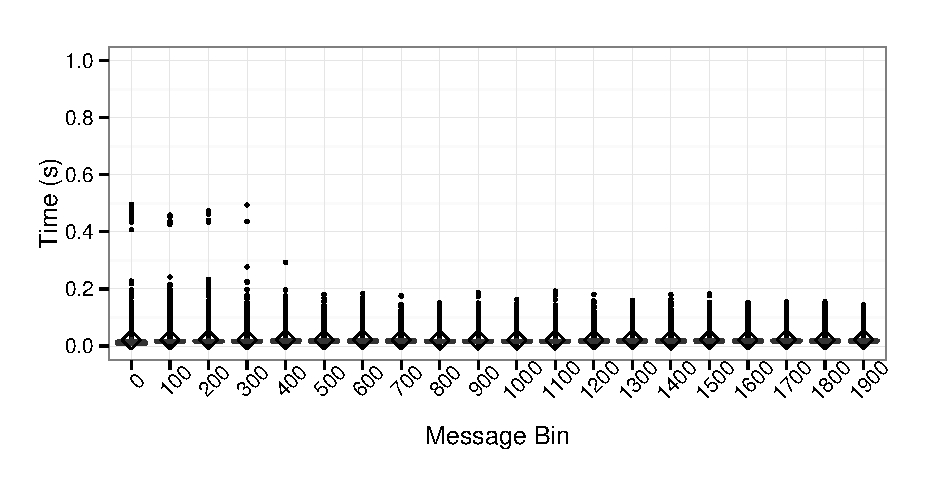
\epsfig{file=figures/parallel/xpilot_ed-8_Time_boxplot_bar_alt.eps,width=0.6\columnwidth}
} \\[-5pt]
%\subfigure[][Single-threaded, $\clusters = \xpilotFineClusterCount$]{
\subfigure[][$\workerCount = 1$]{
\label{fig:xpilot:time:parallel_1_default_fine}
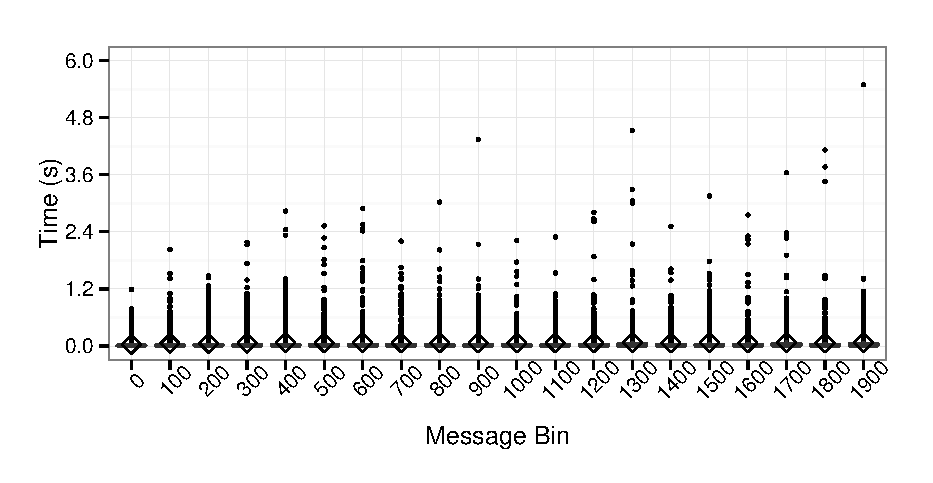
\epsfig{file=figures/parallel/xpilot_ed-1_Time_boxplot_bar_alt.eps,width=0.6\columnwidth}
}
\end{tabular}
\caption[\xpilot parallel verification costs]{\xpilot parallel
  verification costs.
Cross-validation over \xpilotTraces traces.  Boxplot at \xval shows
verification costs for messages \msg{\xval}, $\ldots$, \msg{\xval+99}
in each trace (after training on the other traces).  ``$\Diamond$''
shows the average.}
\label{fig:xpilot:parallel:time}
\end{figure}
\clearpage

\clearpage
\begin{figure}[th]
\centering
\begin{tabular}{c}
%\subfigure[][16 threads, $\clusters = \xpilotFineClusterCount$]{
\subfigure[][$\workerCount = 16$]{
\label{fig:xpilot:delay:parallel_16_default_fine}
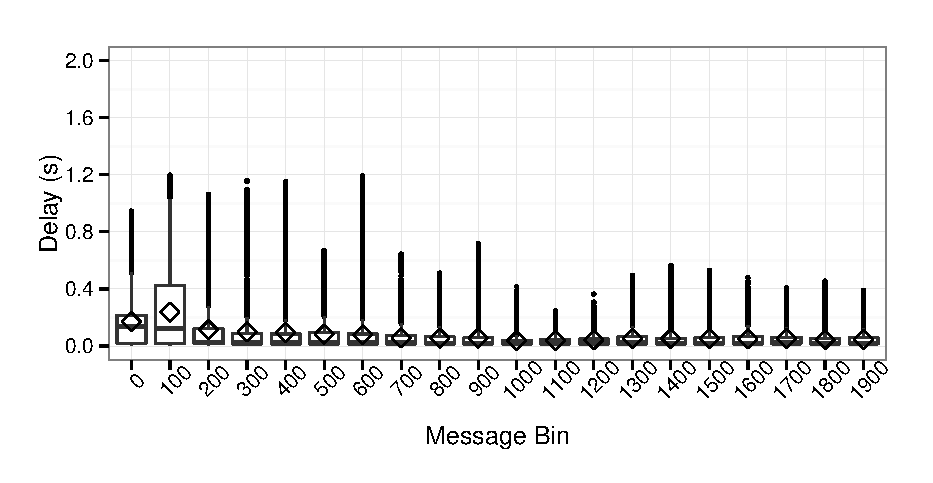
\epsfig{file=figures/parallel/xpilot_ed-16_Delay_boxplot_bar_alt.eps,width=0.6\columnwidth}
} \\[-5pt]
%\subfigure[][8 threads, $\clusters = \xpilotFineClusterCount$]{
\subfigure[][$\workerCount = 8$]{
\label{fig:xpilot:delay:parallel_8_default_fine}
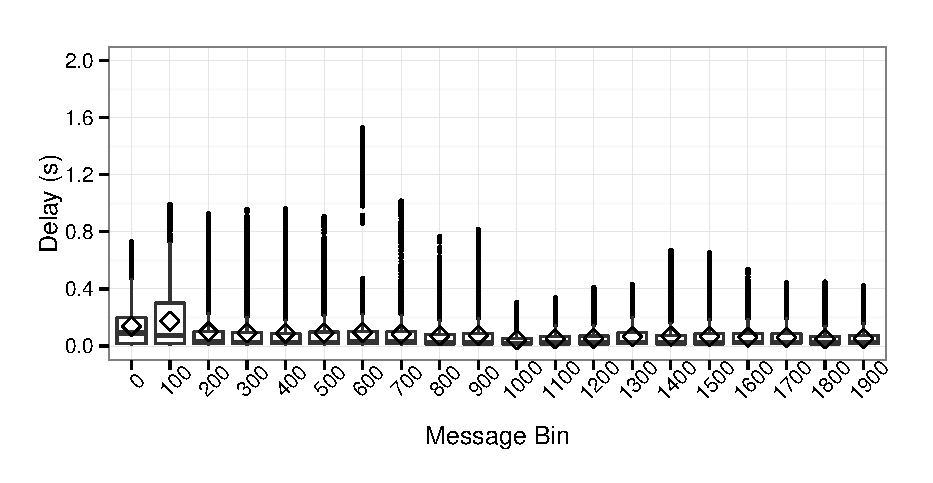
\epsfig{file=figures/parallel/xpilot_ed-8_Delay_boxplot_bar_alt.eps,width=0.6\columnwidth}
} \\[-5pt]
%\subfigure[][Single-threaded, $\clusters = \xpilotFineClusterCount$]{
\subfigure[][$\workerCount = 1$]{
\label{fig:xpilot:delay:parallel_1_default_fine}
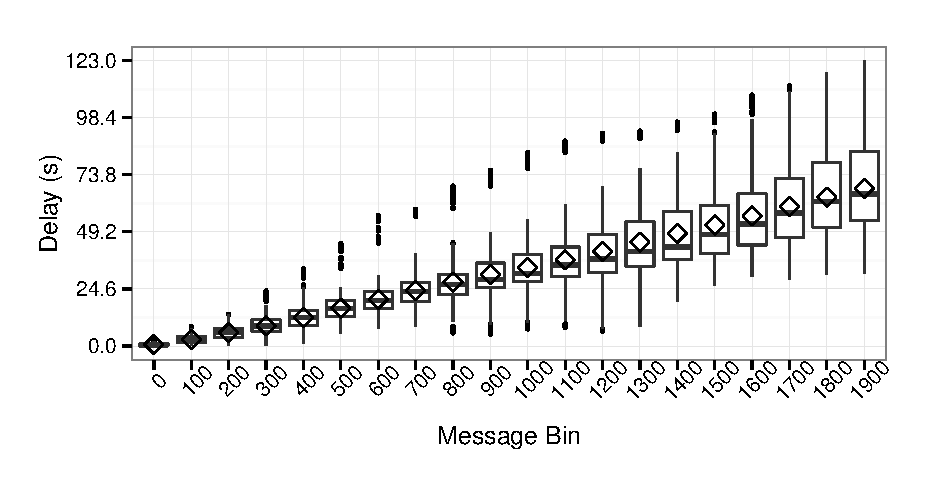
\epsfig{file=figures/parallel/xpilot_ed-1_Delay_boxplot_bar_alt.eps,width=0.6\columnwidth}
}
\end{tabular}
\caption[\xpilot parallel verification delays]{\xpilot parallel
  verification delays.
Cross-validation over \xpilotTraces traces.  Boxplot at \xval shows
verification delays for messages \msg{\xval}, $\ldots$, \msg{\xval+99}
in each trace (after training on the other traces).  ``$\Diamond$''
shows the average.}
\label{fig:xpilot:parallel:delay}
\end{figure}
\clearpage


\begin{figure}[t]
\centering
\begin{tabular}{c}

{\subfigcapskip = 5pt \subfigure[][$\tetrinet$]{
  \small
\begin{tabular}{|r|r|r|}
 \hline
 \multicolumn{3}{|c|}{Cost(s)} \\
 \hline
& \multicolumn{1}{c|}{with } &\multicolumn{1}{c|}{without } \\
& \multicolumn{1}{c|}{\clusterSelector } &\multicolumn{1}{c|}{\clusterSelector } \\
& \multicolumn{1}{c|}{thread} &\multicolumn{1}{c|}{thread} \\
 \hline
%    & ed-8-async-ed\_Cost & ed-8-no-async-ed\_Cost & \\
Min           & 0.0003  & 0.0003   \\
Max           & 16.0291 & 17.1220  \\
Median        & 0.0349  & 0.0221   \\
Mean          & 0.1804  & 0.1833   \\
Std.Dev.      & 1.0507  & 1.2745   \\
\hline
\end{tabular}
} }\\

{\subfigcapskip = 5pt \subfigure[][$\xpilot$]{
  \small
\begin{tabular}{|r|r|r|}
 \hline
 \multicolumn{3}{|c|}{Cost(s)} \\
 \hline
& \multicolumn{1}{c|}{with } &\multicolumn{1}{c|}{without } \\
& \multicolumn{1}{c|}{\clusterSelector } &\multicolumn{1}{c|}{\clusterSelector } \\
& \multicolumn{1}{c|}{thread} &\multicolumn{1}{c|}{thread} \\
 \hline
%    & ed-8-async-ed\_Cost & ed-8-no-async-ed\_Cost & \\
  Min        & 0.0007 & 0.0006  \\
  Max        & 0.4312 & 0.4469  \\
  Median     & 0.0158 & 0.0157  \\
  Mean       & 0.0170 & 0.0172  \\
  Std.Dev.   & 0.0184 & 0.0182  \\
  \hline
\end{tabular}
} } \\

\end{tabular}
\caption[Verification cost with and without \clusterSelector thread]
{Summary of verification cost in seconds for \tetrinet and \xpilot,
with and without a \clusterSelector thread, using $\workerCount = 8$.}
\label{fig:clusterselector}
\end{figure}


\subsection{Evaluation of \nodeScheduler and \clusterSelector Threads}

The parallel algorithm presented in this \paper divides and
distributes the verification computation into separate threads across
multiple CPU cores. Recall in addition to a variable number of
\verifyWorker threads, the algorithm uses two additional threads; one
for the \nodeScheduler procedure (\figref{fig:paralg:sub}) and one for
the \clusterSelector procedure (detailed in \chref{ch:guided}). In this section,
we will examine the performance impact of computing the work done by
the procedures \nodeScheduler and \clusterSelector in separate threads
as opposed to an alternative arrangement where the work is divided
amongst all \verifyWorker threads.

In our current experiments and implementation, the usage of a
\nodeScheduler thread does not provide a measurable performance
benefit. The increased granularity of the workload is offset by the
small overhead of the implementation. Nevertheless, this design
provides a cleaner separation of work for the implementation and we
predict verification of different client software in the future may
benefit from the architecture.

Using a separate thread for the \clusterSelector procedure does
however have a measurable performance impact. The procedure
\clusterSelector is provided a network message \msg{\msgNmbr} and a
set of execution fragments \trainingFrags{}, produced during training
and returns a subset of execution fragments \trainingFrags{\msgNmbr},
used by the \nodeScheduler to inform node selection. The
details of the \clusterSelector algorithm are described in
\chref{ch:guided}.
In our experimental results thus far, each thread has exclusive access
to a CPU core. However, the algorithm is designed so that the
\clusterSelector method can be called synchronously by removing \Spawn
on Line \ref{fig:paralg:spawnClusterSelector} of the
\parallelVerifyAlg procedure in \figref{fig:paralg}. We evaluated this
design decision on the case studies \xpilot and \tetrinet with a new
experimental setup where the \clusterSelector procedure is called
synchronously before the \verifyWorker threads are spawned.
\figref{fig:clusterselector} shows a summary of the verification costs
in seconds for the case studies using $\workerCount = 8$.
The mean verification cost in seconds increases measurably for both
\xpilot and \tetrinet when the verifier is executed without a
\clusterSelector thread.


\section{Evaluation of Optimization Techniques}
\label{sec:par:evalopt}

The performance of parallel symbolic verification is dependent on many
factors. We have shown that a parallel implementation with multiple
worker threads decreases the cost of verification over the
single-threaded implementation outlined in the previous chapters.
Using symbolic execution as the basis for a verification method has
required several optimizations to the underlying implementation, which
have been described in previous chapters. In this section we review
these optimization techniques and evaluate their impact and
interaction with parallel symbolic execution in our case studies.

Several optimization methods were developed and utilized to improve
the performance of symbolic execution for verification. \klee was
designed with techniques for reducing the size and number of queries
that are sent to the underlying constraint solver. One of these
techniques is a cache of solver queries and their respective solver
outputs. Before a constraint formula or query is tested for
satisfiability via \stp, \klee checks a \emph{query cache} and if the
cache contains a hit, the potentially expensive solver operation can
be avoided. If there is a miss, the solver must be instantiated and
the result is added to the cache afterwards. In our implementation,
each worker thread operates a separate solver chain, which means that
\klee query caches are not shared between workers. Additionally,  the
caches are empty upon starting verification of a message sequence. In
the previous chapters, two methods have been demonstrated that enable
better utilization of these caches:
canonicalization~(\secref{sec:guided:eval:results:tetrinet}) and
constraint pruning~(\secref{ssec:scv:approach:pruning}). The
canonicalization method is used to rewrite the variable names in a
solver query before the query cache is checked. The constraint pruning
optimization is used to eliminate variables and formula constructs
that have not been concretized but can be shown to never be relevant
to future branch conditions; variables can be pruned that are no
longer in the scope of execution and are independent from the current
scope.

In this section we evaluate the impact and interactions of parallel
symbolic verification with and without the canonicalization and
constraint pruning optimizations. The experiment operates with
the verifier in three configurations.
The first configuration, which we call \allopt,
is the same configuration used in~\secref{sec:par:eval}, and utilizes
both canonicalization and constraint pruning. The second
configuration, \nocanon, is the same as the former but disables the
canonicalization of queries before the query cache is checked. The
third and final configuration, \noprune, is the same as \allopt
but with constraint pruning disabled. Additionally, we are only
verifying a \emph{single} game play log from each of our case studies,
\xpilot and \tetrinet. Despite using a single log,
the experimental results are representative of
the full case study data sets. The use of a single log
allows easier characterization of the interactions of the optimizations with
symbolic client verification. All of the experiments were performed
with $\workerCount = 16$. If the experiments are configured with
$\workerCount = 1$, disabling canonicalization or constraint pruning
causes the verification to take several hours. In addition to
demonstrating the benefit of constraint pruning and canonicalization,
these results are also useful to characterize the workloads of our
case studies in terms of the symbolic execution optimizations of \klee
and may be of use to others.

\subsection{Impact of Optimizations on Cost and Delay}

\begin{figure}[th]
\centering
{\subfigcapskip = 5pt \subtable[][$\tetrinet$]{
\small
\begin{tabular}{|r|rrr|rrr|}
\hline
& \multicolumn{3}{c|}{Cost (s)}& \multicolumn{3}{c|}{Delay (s)} \\
\hline
& \allopt & \nocanon & \noprune & \allopt & \nocanon & \noprune \\
\hline
Min      & 0.0016 & 0.0014 & 0.0013 & 0.0016 & 0.0014 & 0.0013  \\
Max      & 1.4875 & 3.3591 & 4.7334 & 1.4925 & 3.3690 & 4.7390  \\
Median   & 0.0384 & 0.0376 & 0.0760 & 0.0504 & 0.0467 & 0.1281  \\
Mean     & 0.0835 & 0.0986 & 0.2214 & 0.1387 & 0.1919 & 0.4207  \\
Std. Dev.& 0.1970 & 0.3225 & 0.5242 & 0.2655 & 0.5062 & 0.7522  \\
\hline
\end{tabular}
\label{par:singlecostdelay:tetrinet}
} } \\

{\subfigcapskip = 5pt \subfigure[][$\xpilot$]{
\small
\begin{tabular}{|r|rrr|rrr|}
\hline
& \multicolumn{3}{c|}{Cost (s)}& \multicolumn{3}{c|}{Delay (s)} \\
\hline
& \allopt & \nocanon & \noprune & \allopt & \nocanon & \noprune \\
\hline
Min      & 0.0009 & 0.0007 & 0.0009 & 0.0027 & 0.0086  & 0.0090    \\
Max      & 0.6268 & 0.7627 & 8.2392 & 1.1417 & 55.0549 & 1158.8995 \\
Median   & 0.0171 & 0.0327 & 0.3217 & 0.0266 & 35.5776 & 421.1561  \\
Mean     & 0.0198 & 0.0559 & 0.6080 & 0.1084 & 29.5545 & 537.8276  \\
Std. Dev.& 0.0256 & 0.1213 & 0.7888 & 0.2019 & 16.8834 & 410.7422  \\
\hline
\end{tabular}
\label{par:singlecostdelay:xpilot}
} } \\
\caption{Verification costs and delays for \tetrinet and \xpilot for a
single representative log.}
\label{par:singlecostdelay}
\end{figure}

We now examine the performance interactions of canonicalization and
constraint pruning with parallel symbolic verification. We start with
an experiment to determine the impact of these optimizations on our key
evaluation metrics, cost and delay. \figref{par:singlecostdelay} shows
an overview of the cost and delay times per message during the
verification of a single game play trace from the \tetrinet and
\xpilot case studies. In \figref{par:singlecostdelay:tetrinet} we can
see that for \tetrinet, either disabling the canonicalization
optimization (\nocanon) or disabling the constraint pruning optimization (\noprune)
adversely affects the mean values for cost and delay. The
benefit of these optimizations is even more prevalent in the \xpilot
results shown in \figref{par:singlecostdelay:xpilot}. Disabling
canonicalization increases the mean verification cost by a factor of
five and due to the rapid rate at which \xpilot messages are
transmitted, disabling canonicalization introduces more than a $200
\times$ increase in the mean verification delay. Also, for \xpilot,
constraint pruning is even more important for efficient verification;
the mean verification delay increases from roughly a $0.10$ seconds
with all optimizations to over $8$ minutes without constraint pruning.

\subsection{Impact of Optimizations on Solver Queries}

We can better understand how the canonicalization and constraint
pruning  optimizations impact cost and delay in parallel symbolic
verification by looking at how these optimizations change the
properties of the formulas sent as queries to the constraint solver
(\stp).

\subsubsection{Query Cache Hit Rate}
\figref{par:cachehitrates} shows the overall hit rates of the query
cache in the single log verification experiment and can begin to
explain why the optimizations make verification more efficient.
With all optimizations (\allopt), both \tetrinet and
\xpilot have high hit rates of 99.89\% and 97.13\% respectively. In
other words, of all queries to the constraint solver stack, less than
0.12\% and 3.87\% (\tetrinet and \xpilot, respectively) actually
result in a potentially expensive call to to the constraint solver
\stp. Without the canonicalization optimization (\nocanon), the
effectiveness of the cache is reduced significantly for \tetrinet and
even more so for \xpilot, dropping the hit rate to 33.26\%.

\begin{figure}[t]
\centering
\begin{tabular}{|r|r|r|}
\hline
         & \tetrinet & \xpilot \\
\hline
\allopt  & 0.9989 & 0.9713 \\
\nocanon & 0.6860 & 0.3326 \\
\noprune & 0.9989 & 0.9618 \\
\hline
\end{tabular}
\caption{Overall query cache hit rates for a single log selected from
each of the \tetrinet and \xpilot case studies.}
\label{par:cachehitrates}
\end{figure}

Canonicalization has a large impact on the query cache hit rate
because it reduces the space of variable names that can be found in
the constraint cache. During verification, when a symbolic variable is
generated (e.g., to represent an unknown user input value), in
addition to representing a region of memory, the variable is given a
unique name. The symbolic variable name may be used in a formula to
represent any constraints on any associated symbolic memory region.
Verification in our case studies often generates constraints that have
the same formula structure, but with different variable names. By
canonicalizing the variable names before the query cache is utilized,
the chance of a cache hit becomes much more likely and the expensive
constraint solver query can be avoided. The need for canonicalization highlights a
key difference between the use of symbolic execution for client
verification versus more traditional uses of symbolic execution;
client verification exercises the same paths repeatedly but with
slightly different contexts. Unlike canonicalization, constraint
pruning does not significantly improve the cache hit rate for the case
studies; the \noprune experiment shows the same hit rate for \tetrinet
and only slightly lower hit rate for \xpilot.

\begin{figure}[th]
\centering
\begin{tabular}{c}
\subfigure[][$\tetrinet$]{
\label{par:cachehitratepermessage:tetrinet}
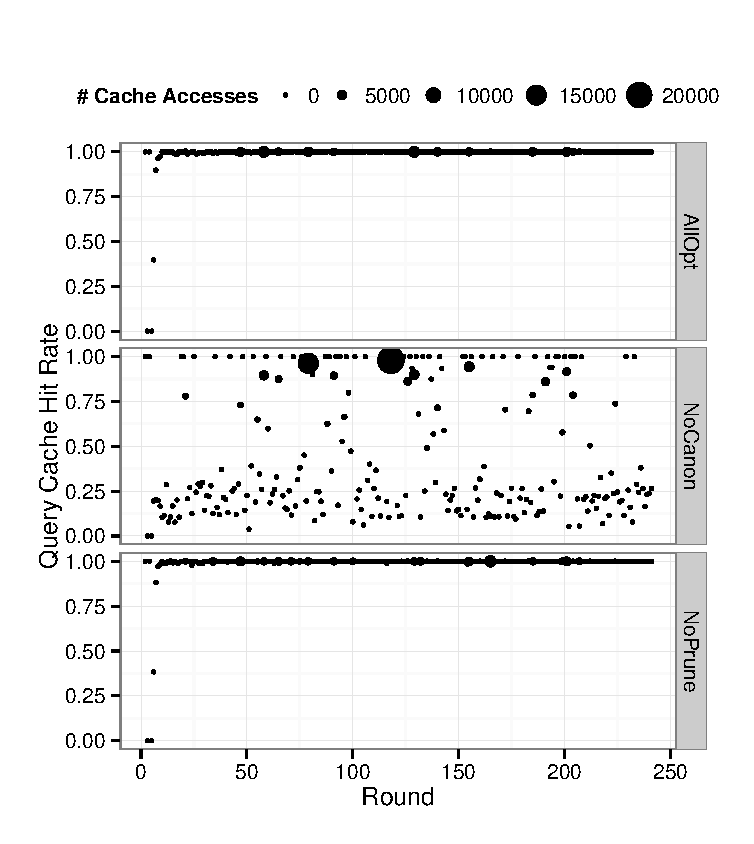
\epsfig{file=figures/parallel/RoundNumbervsQueryCacheHitRate_tetrinet_point_grid_group.eps,width=0.45\columnwidth}
}
\subfigure[][$\xpilot$]{
\label{par:cachehitratepermessage:xpilot}
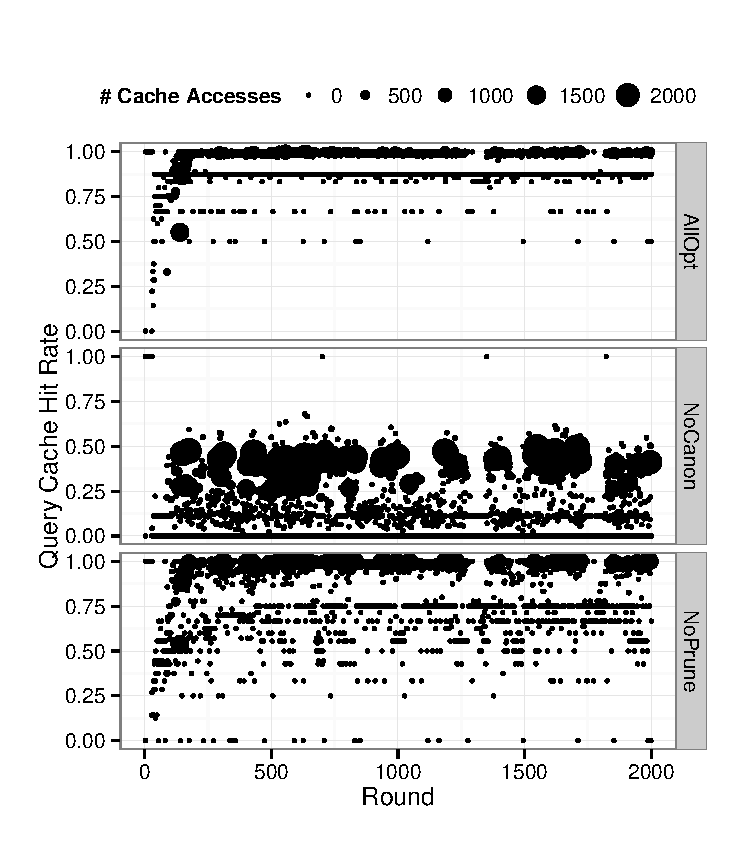
\epsfig{file=figures/parallel/RoundNumbervsQueryCacheHitRate_xpilot_point_grid_group.eps,width=0.45\columnwidth}
}
\end{tabular}
\caption[Query Cache Hit Rates.]{
Query cache hit rates per message for the verification of a single
representative game play log from each of the case studies.
The area of each circle is scaled relative to the
number of cache accesses represented.}
\label{par:cachehitratepermessage}
\end{figure}


\subsubsection{Query Cache Hit Rate Per Message}
\figref{par:cachehitratepermessage} shows the same cache hit rate
values shown in \figref{par:cachehitrates} but \emph{per message}.
\figref{par:cachehitratepermessage} illustrates the change in the
query cache hit rate as verification progresses through the message
log as well as the volume of cache accesses needed to verify each
message. The query cache hit rate is shown on the y-axis and the
message index on the x-axis. Each plotted dot represents the effective
hit rate of the query cache over all queries during the creation of
\execPrefix{\msgNmbr} from \execPrefix{\msgNmbr-1}. The number of
cache accesses needed to construct each \execPrefix{\msgNmbr} is
represented exactly by the area of each circle. The legend shows
several example circle areas and the corresponding number of cache
accesses each area represents. The three configuration types are
indicated on the right side of each plot.

\figref{par:cachehitratepermessage:tetrinet} shows the \tetrinet
experiment. The \allopt and \noprune results are very similar; after
verification of a few messages, the query cache contains enough
entries to produce a very high cache hit rate. However for the
\nocanon configuration, we can observe that without canonicalization
the query cache does not contain entries that match the formulas with
new variables names and is not effective, even towards the end of the
message log.

The \xpilot results are shown in
\figref{par:cachehitratepermessage:xpilot}. The \allopt configuration
for \xpilot shows that verification proceeds for around 30 messages
before the cache hit rate improves significantly. The \noprune
configuration is similar, but with intermittent poor performance due
to the disabling of constraint pruning. Additionally, noticeable bands
appear in the results because of the variety of message types. The
\nocanon plot for \xpilot shows the significance of the
canonicalization optimization, both the query cache hit rate and the
volume of cache accesses are affected with negative impacts on
performance.

\begin{figure}[th]
\centering
\begin{tabular}{c}
\subfigure[][$\tetrinet$]{
\label{par:cachehitcount:tetrinet}
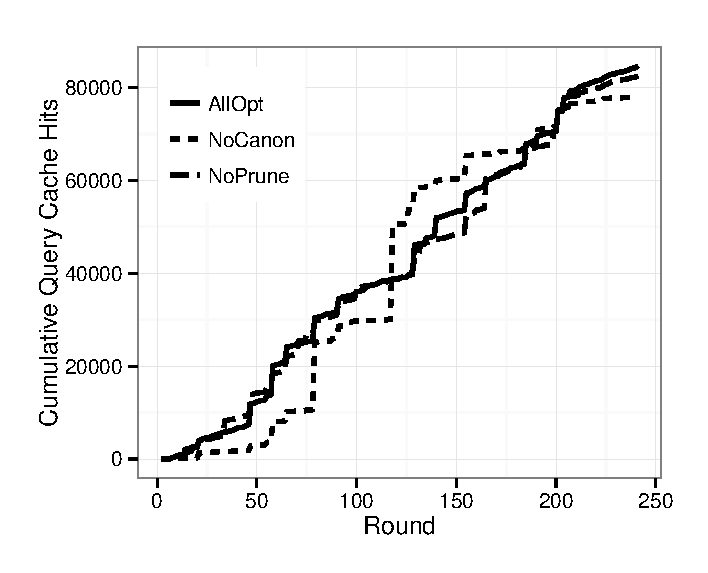
\epsfig{file=figures/parallel/RoundNumbervsCumQueryCacheHits_tetrinet_line_group.eps,width=0.45\columnwidth}
}
\subfigure[][$\xpilot$]{
\label{par:cachehitcount:xpilot}
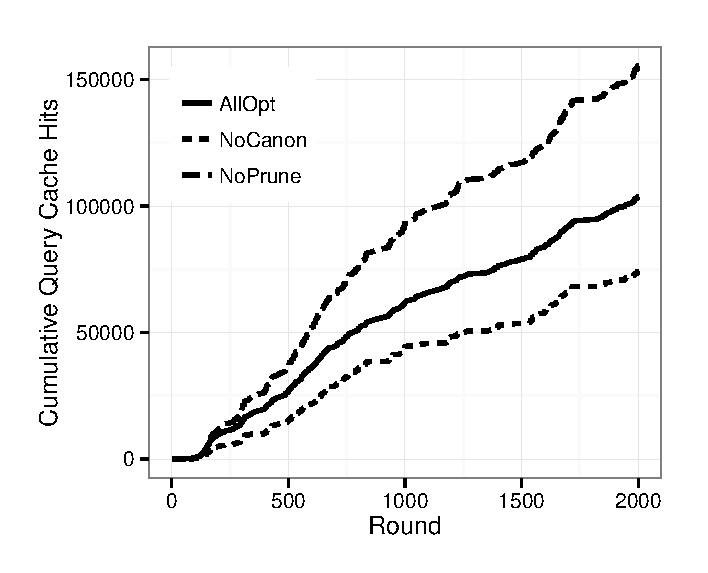
\epsfig{file=figures/parallel/RoundNumbervsCumQueryCacheHits_xpilot_line_group.eps,width=0.45\columnwidth}
}
\end{tabular}
\caption[Cumulative number of cache hits.]{The cumulative number query cache hits over the verification
of a single game play log from \xpilot and \tetrinet.}
\label{par:cachehitcount}
\end{figure}

\subsubsection{Cumulative Query Cache Hits and Solver Queries}
We now examine how the query cache is exercised by the three
configurations in terms of the cumulative number of hits in the query
cache and the cumulative number of misses that lead to actual calls to
the constraint solver. \figref{par:cachehitcount} shows the cumulative
number of query cache hits for \tetrinet and \xpilot over the
verification of a single representative game play log.  By the time
the last message is verified, the \tetrinet experiment results in over
$80,000$ cache hits amongst the 16 worker threads, while the  \xpilot
experiment generates over $100,000$ cache hits. The cumulative number
of final cache hits is about the same for each configuration of
\tetrinet. However for \xpilot there is a significant difference; the
\noprune configuration has approximately twice as many query cache
hits as \nocanon. The \noprune configuration produced more cache hits
overall, even more than \allopt, because the overall search was less
efficient and interacted with the parallel verification.
Under \noprune, each verify worker has a more complex
workload with larger constraints and therefore the time to discover
the correct execution prefix increases. The additional time needed allows
other worker threads to search additional paths, thus increasing the
number of query cache hits. This aligns with the results for the
\noprune configuration in \figref{par:cachehitratepermessage:xpilot};
the relative query cache hit rate is slightly less than \allopt, but
the overall number of cache accesses (indicated by the size of the
circles) is larger.

\begin{figure}[th]
\centering
\begin{tabular}{c}
\subfigure[][$\tetrinet$]{
\label{par:solverqueries:tetrinet}
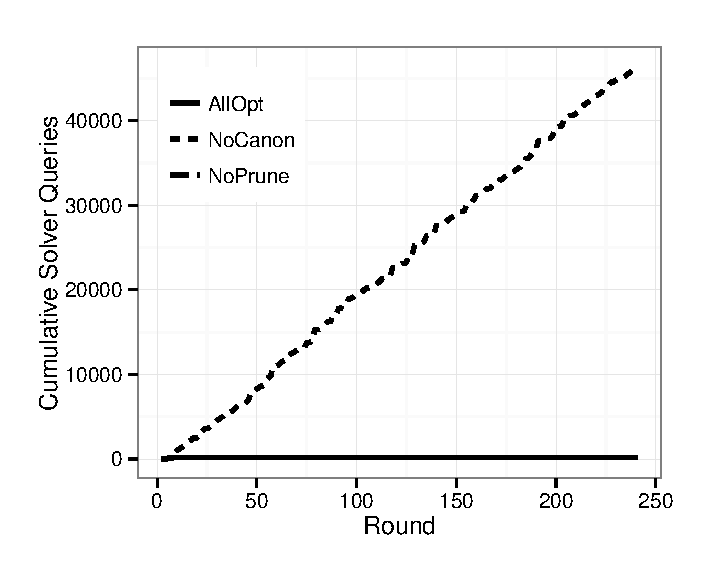
\epsfig{file=figures/parallel/RoundNumbervsCumQueries_tetrinet_line_group.eps,width=0.45\columnwidth}
} %\\[-5pt]
\subfigure[][$\xpilot$]{
\label{par:solverqueries:xpilot}
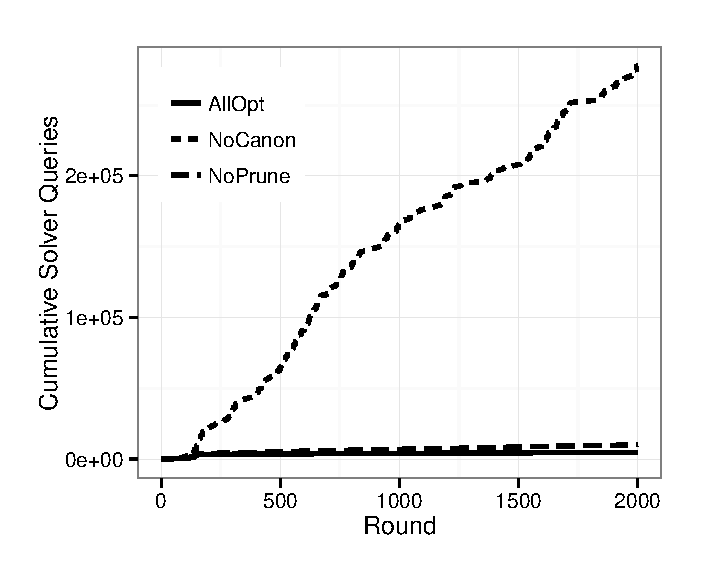
\epsfig{file=figures/parallel/RoundNumbervsCumQueries_xpilot_line_group.eps,width=0.45\columnwidth}
} %\\[-5pt]
\end{tabular}
\caption[Cumulative number of solver queries.]{The cumulative number
  of queries to the solver (\stp) over the verification of a single game play log
from \xpilot and \tetrinet.}
\label{par:solverqueries}
\end{figure}

A query is only made to the constraint solver \emph{after} a query
cache miss has occurred. Therefore, the number of misses in the caches
is exactly equal to the number of actual queries made to the
constraint solver. \figref{par:solverqueries} shows the cumulative
number of queries to the constraint solver (\stp) over the
verification of single game log for both \tetrinet and \xpilot using
the three different configurations. Here it is very evident that for
both case studies, the canonicalization optimization significantly
reduces the overall number of expensive queries to \stp. If we combine
the overall numbers for \tetrinet from
\figref{par:solverqueries:tetrinet} and
\figref{par:cachehitcount:tetrinet},
we can see that \nocanon had
a significantly greater number of solver queries, including queries
resulting in a cache hit. Again, this is due to an interaction with
workers operating in parallel; the time to discover a valid execution
prefix increases when more time is spent in the constraint solver.
Therefore, other worker threads explore additional paths, leading to
a greater number of client instructions executed across all worker
threads. The impact of this interaction is examined further in the
next section~ (\ref{sec:par:optinst}).

\begin{figure}[th]
\centering
\begin{tabular}{c}
\subfigure[][$\tetrinet$]{
\label{par:querysize:tetrinet}
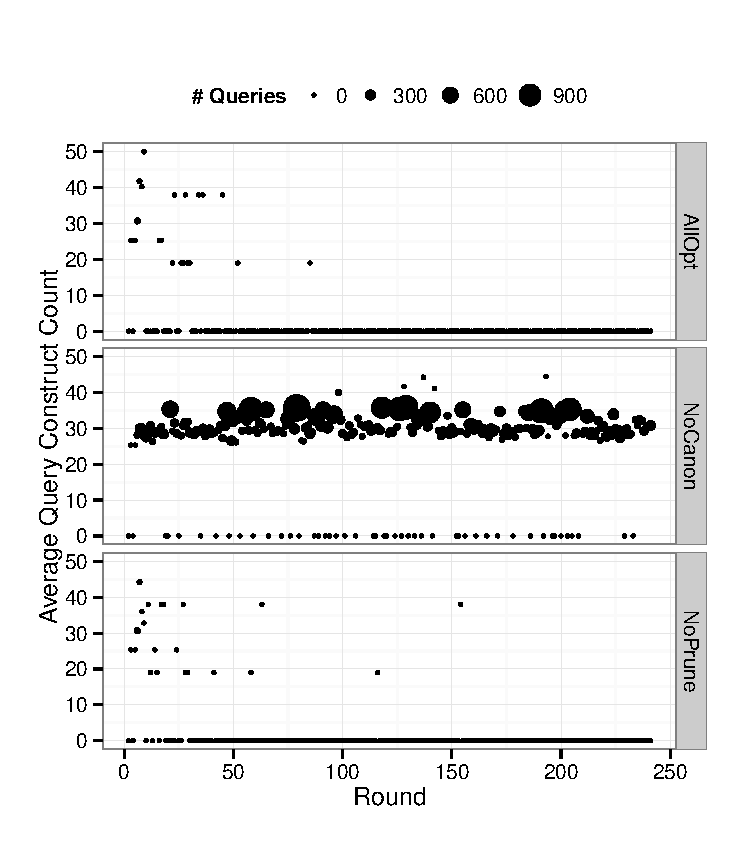
\epsfig{file=figures/parallel/RoundNumbervsAverageQueryConstructs_tetrinet_point_grid_group.eps,width=0.45\columnwidth}
}
\subfigure[][$\xpilot$]{
\label{par:querysize:xpilot}
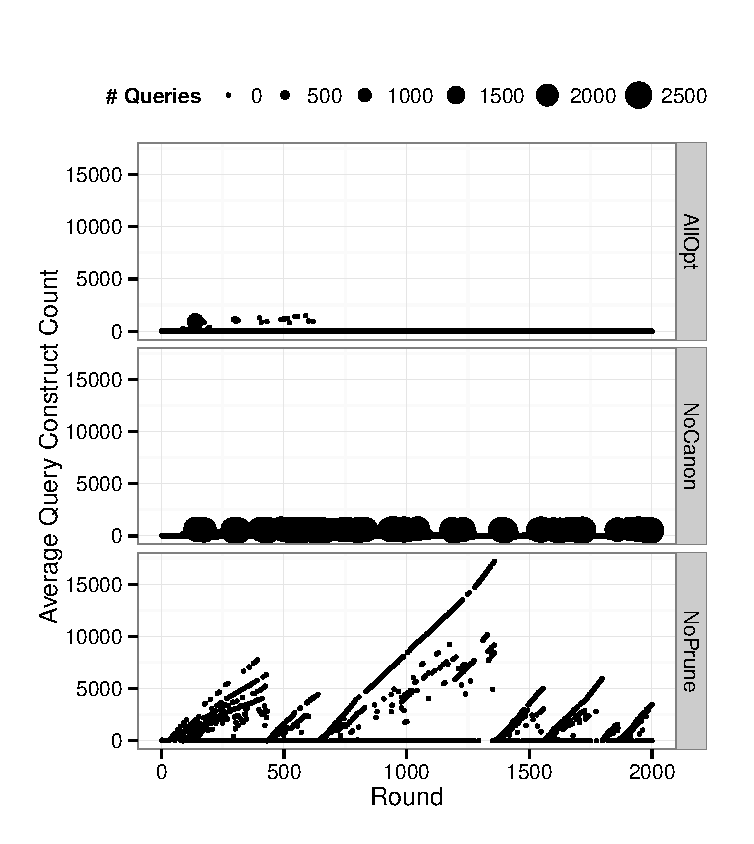
\epsfig{file=figures/parallel/RoundNumbervsAverageQueryConstructs_xpilot_point_grid_group.eps,width=0.45\columnwidth}
}
\end{tabular}
\caption[Complexity of Solver Queries.]{
Average query construct count per message
verified in a single representative game play log from \tetrinet and
\xpilot.
The area of each circle is scaled relative to the
number of solver queries represented.}
\label{par:querysize}
\end{figure}

\subsubsection{Complexity of Solver Queries}
In addition to the number of queries to the constraint solver, we also
characterize the complexity of these queries in terms of the size of
the queried constraint. A constraint formula consists of binary and
unary operators on variables or concrete values; each of those
operators is counted as a single construct. The metric we use for size
is a measure that corresponds to the number constructs in the query.
Each circle plotted in \figref{par:querysize} summarizes the
complexity of the constraint formulas sent to the solver by showing
the average number of constructs in the solver queries during the
creation of \execPrefix{\msgNmbr} from \execPrefix{\msgNmbr-1}.
Additionally, the area of each circle represents the number of
queries sent to the constraint solver. Note that the data shown
in \figref{par:querysize} characterizes the query formulas sent to
the constraint solver (STP) after a query cache miss has occurred.

As we have seen, the lack of canonicalization leads to poor cache
utilization; the effects of which are twofold for the \nocanon
configuration in \figref{par:querysize:tetrinet}. First, the average
query construct count (on the y-axis) is greater than \allopt across
the message sequence. Without canonicalization, fewer
queries are located in the query cache and thus more queries are sent
to the constraint solver and these queries have a greater
query construct count. Second, the total number of
queries is greater (area of circles) because poor cache utilization
leads to a greater number of client instructions executed; this is
examined further in the next section (\ref{sec:par:optinst}).

The \xpilot experiment in \figref{par:querysize:xpilot} reveals
similar results for the \nocanon configuration. The average query
construct count (on the y-axis) is greater than \allopt across the
message sequence because larger queries are not located in the cache
and the total number of queries is larger (area of circles) because a
greater number of client instructions are executed. In the \noprune
configuration, there is a behavior where the average number of
constructs increases with each creation of \execPrefix{\msgNmbr} from
\execPrefix{\msgNmbr-1}, with a periodic ``reset'' of the average
constraint complexity. This behavior is seen when constraint pruning
is disabled because independent constraints that contain symbolic
variables that are generated for \execPrefix{\msgNmbr}, may have a
relationship with a symbolic variable generated during the creation of
\execPrefix{\msgNmbr-1}. For example, suppose a symbolic variable
represents the current time and is fully symbolic. This variable will
be strictly greater than a similar variable that represents an
earlier instance of the time. These constraints do not grow throughout
the entire gameplay session because of high level game events that
cause, for example, a reset of certain game state values. By using the
constraint pruning techniques that are described in the previous
chapter, the complexity of solver queries can be dramatically reduced
and can be seen clearly in \figref{par:querysize:xpilot} by comparing
\allopt and \noprune.

\subsection{Impact of Optimizations on Instructions Executed and Memory Usage}
\label{sec:par:optinst}

%\begin{table}[ht]
%\centering
%\begin{tabular}{rrrr}
%\hline
%% & No-Canonicalization\_InstructionCount & No-Pruning\_InstructionCount & All-Opt\_InstructionCount \\
%               & \nocanon       & \noprune       & \allopt \\
%\hline
%
%Min            & 61.0000        & 61.0000        & 61.0000             \\
%Max            & 77361709.0000  & 26033093.0000  & 23564623.0000       \\
%Median         & 211246.0000    & 276570.0000    & 369236.5000         \\
%Mean           & 1413244.8667   & 1150238.6250   & 1141894.7417        \\
%Std.Dev        & 6630185.9084   & 3160070.1607   & 3323343.5091        \\
%Sum            & \num{3.39e8} & \num{2.76e8} & \num{2.74e8}      \\
%
%%Min            & 61.0000        & 61.0000        & 61.0000             \\
%%Max            & 77361709.0000  & 26033093.0000  & 23564623.0000       \\
%%Median         & 211246.0000    & 276570.0000    & 369236.5000         \\
%%Mean           & 1413244.8667   & 1150238.6250   & 1141894.7417        \\
%%Std.Dev        & 6630185.9084   & 3160070.1607   & 3323343.5091        \\
%%Sum            & 339178768.0000 & 276057270.0000 & 274054738.0000      \\
%
%\hline
%\end{tabular}
%\end{table}

We now examine the impact of canonicalization and constraint
pruning on two additional performance metrics in the verifier. The
number of \emph{client} instructions executed during symbolic
execution by the verifier and the memory utilization of the verifier.

The number of client instructions executed characterizes the work done
by the symbolic execution component of the verifier. The lower bound
on the number of client instructions executed up to verification of
message \msgNmbr is the length of the execution prefix
$\execPrefix{\msgNmbr}$. In practice though, the number of client
instructions executed by the verifier is much greater than the lower
bound. In fact, achieving this lower bound is likely not possible
without knowledge of the remote client state and remote user inputs.
A key objective in the design of our verifier was to reduce the total
number of client instructions executed during the creation of
\execPrefix{\msgNmbr} from \execPrefix{\msgNmbr-1}, thus lowering the
verification cost. \chref{ch:guided} outlines techniques to reduce the
number of client instructions executed using edit distance based node
selection and training data. Executing client instructions is not,
however, the only work of the verifier. \figref{fig:time_summary} in
\chref{ch:guided} gives a high-level view of the time spent in each
component of the verifier and shows that a significant percentage of
the verifier's computation is spent doing work other than executing
instructions, e.g., solving constraints. Canonicalization and
constraint pruning do not \emph{directly} affect the number of client
instructions executed, but may decrease the time of constraint
solving. In fact, when the verifier is configured with $\workerCount =
1$, under each of the configurations \allopt, \nocanon and \noprune,
the verifier will execute the exact same number of client
instructions. However, when $\workerCount > 1$, any change to the
performance of the verifier can affect the total number of client
instructions executed amongst the verify worker threads. The
interaction between the performance of constraint solving and the
total number of client instructions executed is complex. For example,
by decreasing the time spent constraint solving, nodes may be
``revealed'' more quickly in the node tree, leading to quicker
utilization of all \verifyWorker threads, and therefore a greater
number of instructions executed. Conversely, more expensive constraint
solving may also lead to an increased number of client instructions
executed. This is because if the time taken to create
\execPrefix{\msgNmbr} by one \verifyWorker thread is increased, other
\verifyWorker threads may execute additional client instructions.
Another important point regarding the relationship between
verification cost and client instructions executed is that when the
verifier is configured with $\workerCount > 1$, verification costs
should be lower than a verifier configured with $\workerCount  = 1$,
as seen in our earlier evaluation, despite potentially executing a
greater number of client instructions.

\begin{figure}[t]
\centering
\begin{tabular}{c}
\subfigure[][$\tetrinet$]{
\label{par:instcount:tetrinet}
\epsfig{file=figures/parallel/RoundNumbervsCumInstructionCount_tetrinet_line_group.eps,width=0.45\columnwidth}
} %\\[-5pt]
\subfigure[][$\xpilot$]{
\label{par:instcount:xpilot}
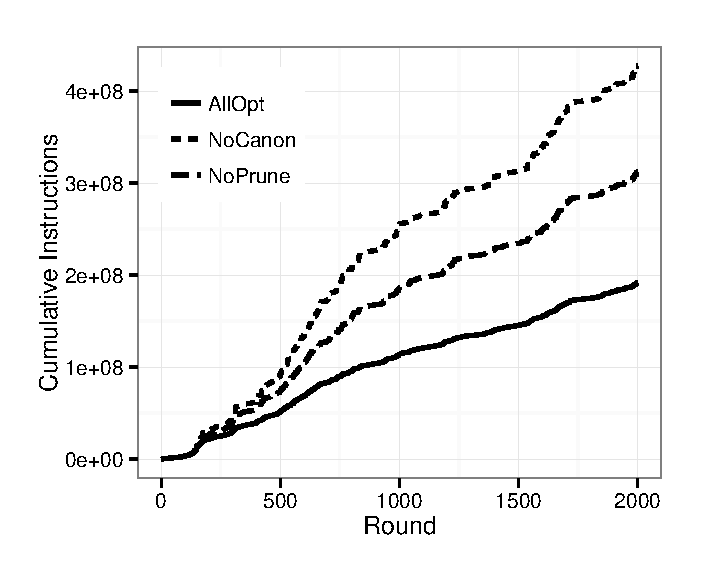
\epsfig{file=figures/parallel/RoundNumbervsCumInstructionCount_xpilot_line_group.eps,width=0.45\columnwidth}
} %\\[-5pt]
\end{tabular}
\caption[Client instructions executed.]{Cumulative number of client instructions executed per message during
during verification of a single representative game play log from the
\tetrinet and \xpilot case studies.}
\label{par:instcount}
\end{figure}

Figure~\ref{par:instcount} shows the cumulative number of client
instructions executed over the verification of a single representative
game play log from \tetrinet and \xpilot under the three
configurations. In the \allopt configuration, for \tetrinet and \xpilot,
the total number of client instructions executed is
\num{2.7e8} and \num{1.9e8} respectively. As before, the verifier was
configured with $\workerCount = 16$ for these results.

The \tetrinet client contains more possible execution paths than the
\xpilot client; therefore worker utilization is high when a message
is verified.
With high worker utilization, disabling
canonicalization or constraint pruning increases the overall cost of
executing a client instruction on average and sometimes decreases the
total number of client instructions executed. This explains the
regions in \figref{par:instcount:tetrinet}, where the \nocanon or
\noprune lines are below the \allopt line.
During verification of the \xpilot client, utilization of the
\verifyWorker threads is not always 100\%, therefore in the \nocanon and
\noprune configurations, the increased verification cost of a single
message enables better utilization of all \verifyWorker threads.
Better thread utilization allows exploration of additional paths and
execution of additional client instructions.
\figref{par:instcount:xpilot} shows the increase in cumulative client
instructions executed for \nocanon and \noprune.
If more client instructions are executed, there is a corresponding
increase in the number of solver queries, which helps explain why
disabling canonicalization and constraint pruning led to an increase
in the number of cache hits and solver queries seen in
\figref{par:cachehitcount} and
\figref{par:solverqueries}.

\begin{figure}[t]
\centering
\begin{tabular}{c}
\subfigure[][$\tetrinet$]{
\label{fig:memory:tetrinet}
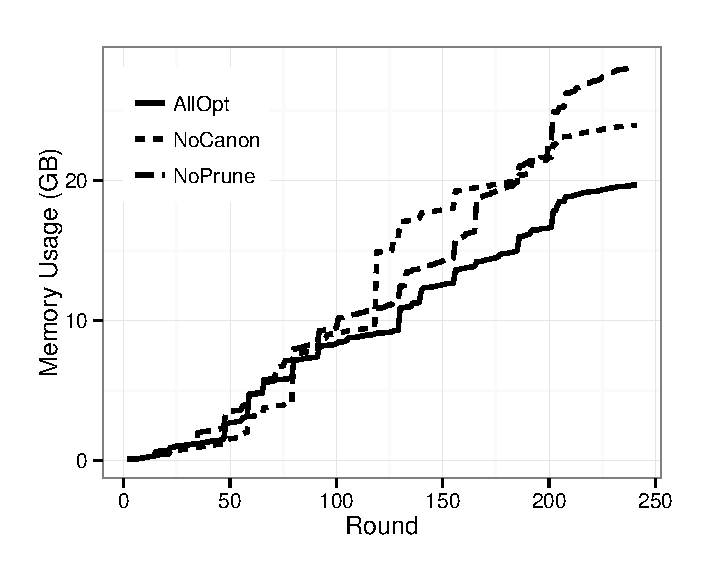
\epsfig{file=figures/parallel/RoundNumbervsMemoryUsage_tetrinet_line_group.eps,width=0.45\columnwidth}
} %\\[-5pt]
\subfigure[][$\xpilot$]{
\label{fig:memory:xpilot}
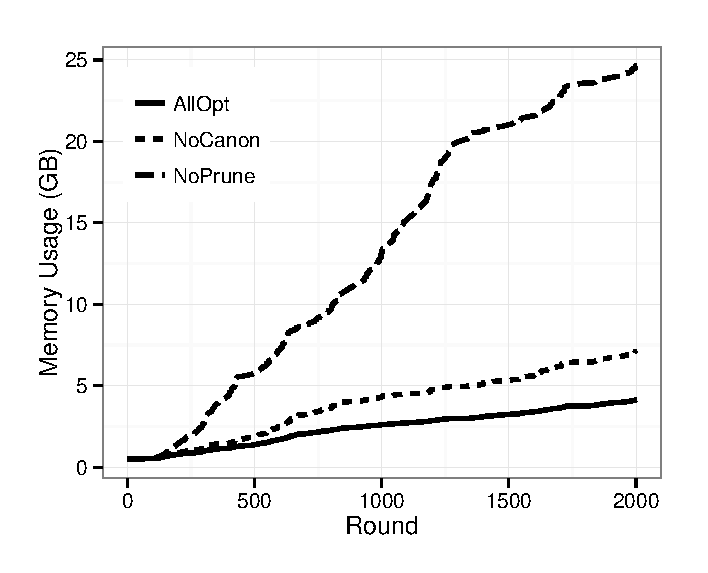
\epsfig{file=figures/parallel/RoundNumbervsMemoryUsage_xpilot_line_group.eps,width=0.45\columnwidth}
} %\\[-5pt]
\end{tabular}
\caption[Parallel verifier memory usage.]{
Cumulative overall memory utilization in gigabytes
during verification of a single representative game play log for the
\tetrinet and \xpilot case studies.}
\label{fig:memory}
\end{figure}

\section{Summary}

In this \paper we described a parallel client verification
algorithm that vastly reduces verification costs for our case study
applications, \xpilot and \tetrinet. Improving the verification cost
using a parallel algorithm pays large dividends when accumulated over
time; in some cases the delays drop from 2 minutes to less than 2
seconds. To achieve these results, we designed and implemented a
multi-threaded client verification algorithm that uses multiple
threads to enable concurrent exploration of execution paths.
These results open the door to using symbolic client verification on
the critical path of serving client requests and could provide a new
method for preventing malicious clients from disrupting gameplay
and damaging server infrastructure. 

